%initialising document, adjust papersize, fontsize and page orientation to your needs
\documentclass[a4paper, fontsize = 8pt, landscape]{scrartcl}
\usepackage{layout_and_colours}
\title{Kommunikationstechnik}
\author{Jil Zerndt}
\date{FS 2024}

\createtitlepagestyle
\createmainpagestyle

\begin{document}
\begin{multicols*}{3}
    \thispagestyle{TitlePageStyle}
		\maketitle
    \input{1_Übertragungsmedien}
    \raggedcolumns
    %\newpage
    \section{OSI Referenzmodell}
    \subsubsection{Schichten, Protokolle und Dienste}
    \begin{definition}{Systeme}
        Offene Systeme (im Gegensatz zu proprietären Systemen) basieren auf öffentlich verfügbaren Standards für Schnittstellen und Protokolle
    \end{definition}

    \begin{definition}{Dienst}
        sendet und empfängt bestätigte und unbestätigte Daten.
    \end{definition}
    \begin{highlight}{Klassifizierung von Diensten}
    \begin{center}
        \begin{minipage}{0.46\linewidth}
                \tcbsubtitle{Verbindungsorientiert}
                    \begin{itemize}
                        \item Verbindungsaufbau nötig
                        \item Informationen vom Empfänger - Optionen aushandeln
                        \item Reihenfolge der Daten bleibt erhalten
                    \end{itemize}
                \tcbsubtitle{Verbindungslos}
                \begin{itemize}
                    \item Jederzeit (send and forget)
                    \item Ziel muss nicht bereit sein
                    \item einfacher umzusetzen
                \end{itemize}
        \end{minipage}
        \hfill\vline\hfill
        \begin{minipage}{0.47\linewidth}
            \tcbsubtitle{Zuverlässig}
                \begin{itemize}
                    \item Kein Datenverlust
                    \item Sicherung durch Fehler-Erkennung/-Korrektur
                    \item Text-Nachrichten
                \end{itemize}
            \tcbsubtitle{Unzuverlässig}
            \begin{itemize}
                \item Möglicher Datenverlust
                \item Keine Sicherung
                \item Streaming
            \end{itemize}
        \end{minipage}
    \end{center}
\end{highlight}

\begin{definition}{Schicht}
    hat die Aufgabe der darüberliegenden Schicht bestimmte Dienste zur Verfügung zu stellen. Die Schichten benötigen kein Wissen über die Realisierung der darunterliegenden Schicht.
\end{definition}

\begin{definition}{Protokoll}
     eine Sammlung von Nachrichten, Nachrichtenformaten und Regeln zu deren Austausch.\\
     In der Technik ist ein Kommunikationsprotokoll eine Vereinbarung, die festlegt wie eine Datenübertragung zwischen Kommunikationspartnern abläuft.
\end{definition}

\columnbreak

\subsubsection{Datenübertragung und Schichtenmodell}

\begin{concept}{OSI Modell}
    \begin{itemize}
        \item Referenzmodell, beschreibt Kommunikation zwischen räumlich entfernten Kommunikationspartnern
        \begin{itemize}
            \item 7 Schichten (unabhängige Teilfunktionen)
            \item Eine Schicht erfüllt, mit Hilfe der untergeordneten Schichten, bestimmte Aufgaben und bietet der übergeordneten Schicht über eine definierte Schnittstelle einen definierten Dienst an
            \item Gleiche Schichten in verschiedenen Systemen kommunizieren nach den Regeln eines standardisierten Protokolls
        \end{itemize}
        \item Die Kommunikation erfolgt logisch zwischen Protokollimplementierungen auf gleicher Schicht (Kommunikationsbeziehung), physikalisch wandern die Daten beim Sender im Stack «nach unten», werden über ein Medium übertragen, und wandern beim Empfänger wieder «nach oben»
    \end{itemize}
\end{concept}

\begin{definition}{OSI Layers}
    \begin{itemize}
        \item Anwendungsschichten 5-7
        \begin{itemize}
            \item Lösen allgemeine Aufgaben
        \end{itemize}
        \item Transportschichten
        \begin{itemize}
            \item Teil des Betriebssystems und Treiber
            \item «Socket»-Schnittstelle für eigene Anwendungsprotokolle
        \end{itemize}
    \end{itemize}
\end{definition}

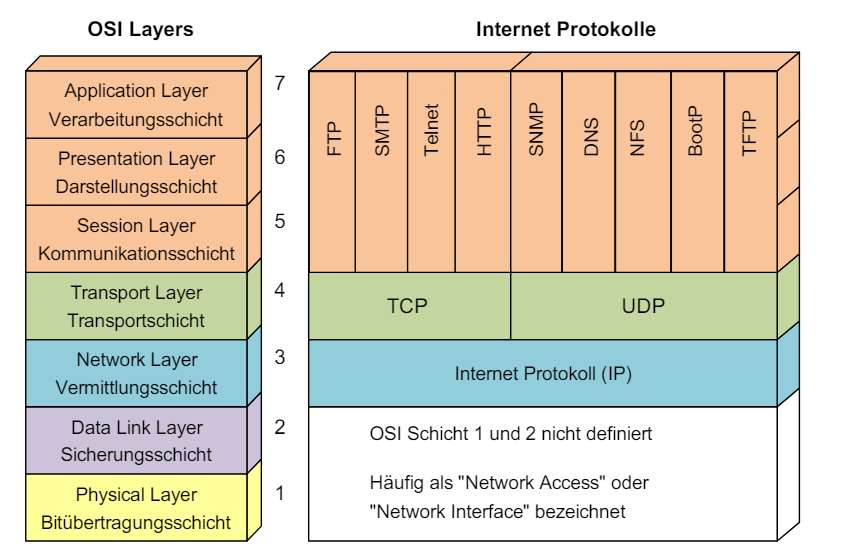
\includegraphics[width=0.9\linewidth]{images/OSI_Modell.png}
\includegraphics[width=0.8\linewidth]{images/Datenübertragung_Schichtenmodell.png}




 
    
 
    \raggedcolumns
    %\newpage
    \section{Physical Layer}
\paragraph{Schicht 1: Bitübertragungsschicht}
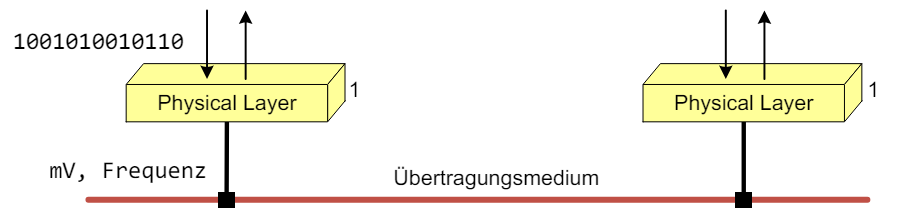
\includegraphics[width=0.75\linewidth]{images/Physical_Layer.png}
\begin{definition}{Funktionalität}\\
    Der Physical Layer sorgt für die ungesicherte Übertragung eines Bit-Stroms zwischen zwei Systemen\\
    Die Standardisierung umfasst:
\begin{itemize}
    \item Elektrische Eigenschaften (Signalform, Amplituden, Frequenzen etc.)
    \item Codierung (Abbildung der Daten auf elektrische Signale)
    \item Mechanische Eigenschaften (Stecker, Pinbelegung etc.)
\end{itemize}
\end{definition}

\begin{remark}
    Verschiedene Übertragungsmedien:
    \begin{itemize}
        \item Koaxialkabel, Twisted Pair, Lichtwellenleiter
        \item Radiowellen
    \end{itemize}
\end{remark}

\subsubsection{Verkehrsbeziehung und Kopplung}
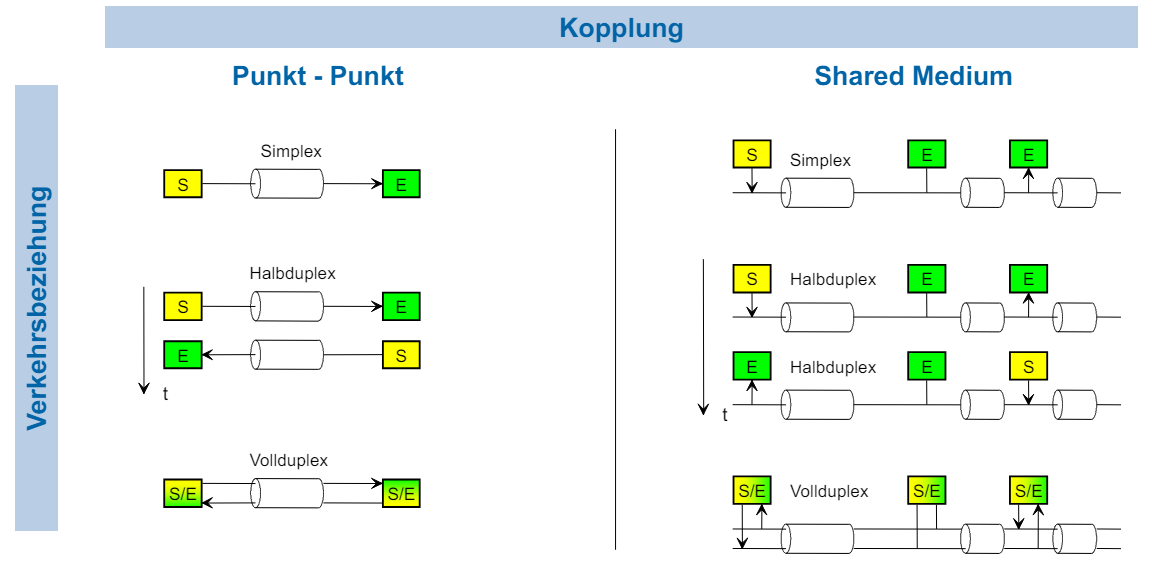
\includegraphics[width=1\linewidth]{images/Verkehrsbeziehung_Kopplung.png}
\begin{concept}{Arten der Kommunikation (Verkehrsbeziehung)}
    \begin{itemize}
        \item Simplex: Ein Kanal, eine Richtung
        \item Halbduplex: Ein Kanal, abwechslungsweise in 2 Richtungen
        \item Vollduplex: Ein Kanal pro Richtung
    \end{itemize}
\end{concept}

\begin{concept}{Arten der Verbindungen (Kopplung)}
    \begin{itemize}
        \item Punkt-Punkt: Direkte Verbindung zweier Kommunikationspartner
        \item Shared Medium: Mehrere Partner verwenden das gleiche Medium
    \end{itemize}
\end{concept}

\columnbreak

\subsection{Übertragungsverfahren: Parallel und Seriell}

\begin{definition}{Parallel vs Seriell}
    \begin{itemize}
        \item Parallele Übertragung: mehrere Bits gleichzeitig über mehrere Leitungen
        \item Serielle Übertragung (dominierend): einzelne Bits zeitlich gestaffelt
    \end{itemize}
    Bei der seriellen Übertragung wird weiter unterschieden zwischen seriell synchroner und
    seriell asynchroner Übertragung
\end{definition}

\begin{definition}{Serielle asynchron Übertragung}\\
    Zwischen Sender und Empfänger werden folgende Abmachungen benötigt:
    \begin{itemize}
        \item Bitrate
        \item Anzahl Datenbits (Typisch 1 Byte)
        \item Anzahl Stoppbits (Typisch 1 Bit)
    \end{itemize}
    Taktrückgewinnung ist möglich
\end{definition}

\begin{example}
    \includegraphics[width=1\linewidth]{images/serielle_asynchrone_übertragung.png}
    Welcher Wert / welches Zeichen wird hier übertragen?
    \begin{itemize}
        \item Empfangen wird 1001 1100 – LSB first –> 0011 1001 (binär); 0x39 (hex); ASCII Code 57 = «9»
    \end{itemize}
    Was ist die Genauigkeitsanforderung an die Takte von Sender und Empfänger (geometrisch
    ausgedrückt)?
    \begin{itemize}
        \item Letzte Abtastung muss noch im Zeitfenster liegen (Stop-Bit bei einem Stop-Bit); also ½T auf 9½ T
    \end{itemize}
\end{example}

\begin{KR}{Clock Drift}\\
    Maximale Framegrösse Ethernet: 1’500 Bytes.
    \begin{itemize}
        \item Standard: Oszillatoren brauchen Genauigkeit von ±50 ppm 
        \item 50 ppm (parts per million) $\rightarrow$ Fehler von 0.00005
        \item Worst-Case: Sender Fehler = -50 ppm, Empfänger Fehler = +50 ppm (oder umgekehrt)
    \end{itemize}
    \textcolor{pink}{Sicheres Abtasten von Daten?} (im Worst-Case)
    \begin{itemize}
        \item 1'500 Bytes = 12'000 Bit; $T_{Bit}$ = 1 Bit-Zeit
        \item 100ppm Differenz Sender/Empfänger $\rightarrow 100 * 10^{-6} = 1 * 10^{-4}$
        \item Fehler pro Bit: $10^{-4} T_{Bit}$
        \item 1’500 Bytes sind $12’000 = 1.2 * 10^4$ Bit
        \item Die Abweichung ist somit $1.2 * 10^4 \text{Bit} * 10^{-4} T_{Bit} / \text{Bit} = 1.2 T_{Bit}$
        \item fehlerfreie Abtastung nicht möglich (ohne weitere Massnahmen)
    \end{itemize}
\end{KR}

\columnbreak

\begin{definition}{Serielle synchron Übertragung}\\
    Bei der synchronen Übertragung arbeitet der Empfänger mit dem gleichen Takt wie der Sender
    \begin{itemize}
        \item Keine Start- und Stoppbits benötigt
        \item Der Takt muss zusätzlich übertragen werden
    \end{itemize}
    Die Übertragung des Takts erfolgt über ein Codierungsverfahren oder eine zusätzliche Leitung. \\
    Es ist die Aufgabe vom Data Link Layer die Grenzen der einzelnen Bytes zu ermitteln (Preamble, etc.)
\end{definition}

\begin{example}
    \includegraphics[width=0.8\linewidth]{images/serielle_synchron_Übertragung.png}\\
    Welches Bit vom obigen Diagramm trifft zuerst beim Empfänger ein (1/0)? "1"\\
    \textbf{Vorsicht, wenn Weg und Zeit im selben Bild gezeichnet sind.}
\end{example}

\begin{concept}{Synchrone Übertragung ohne separate Taktleitung}\\
    Geeignete Codierverfahren erlauben den Takt zusammen mit dem Datensignal zu übertragen (Leitungscode)\\
    \includegraphics[width=0.9\linewidth]{images/synchrone_übertragung_ohne_seperate_Taktleitung.png}\\
    Unter Codierung versteht man hier die Umsetzung der Einsen und Nullen auf eine physikalische Grösse
    \begin{itemize}
        \item Vorteil: Es wird nur eine Leitung benötigt
        \item Nachteil: Zusätzlich 2 x Leitungseinrichtung
    \end{itemize}
\end{concept}


\subsection{Leitungscodes}

\begin{definition}{Leitungscodes und Taktrückgewinnung}\\
    Mittels Leitungscode ist es dem Empfänger möglich den Takt heraus zu extrahieren (keine 2. Leitung nötig)\\
    \includegraphics[width=1\linewidth]{images/taktrückgewinnung_prinzip.png}
\end{definition}

\begin{theorem}{Anforderungen Leitungscodes}
\begin{itemize}
    \item die physikalisch vorhandene Bandbreite effizient nutzen
    \item Taktrückgewinnung erlauben (keine separate Taktleitung nötig)
    \item möglichst gleichspannungsfrei sein, um Sender und Empfänger mit Übertragern (Signaltransformatoren, Magnetics) galvanisch trennen zu können.
\end{itemize} 
\end{theorem}

\begin{example}
    Wie könnte man Gleichspannungsfreiheit und galvanische Isolation in einem Schritt erreichen?
    \begin{itemize}
        \item Z.B. durch den Einsatz von Lichtwellenleitern
    \end{itemize}
\end{example}

\begin{concept}{AMI Leitungscode}\\
    3-wertiger AMI-Code (Alternate Mark Inversion)\\
    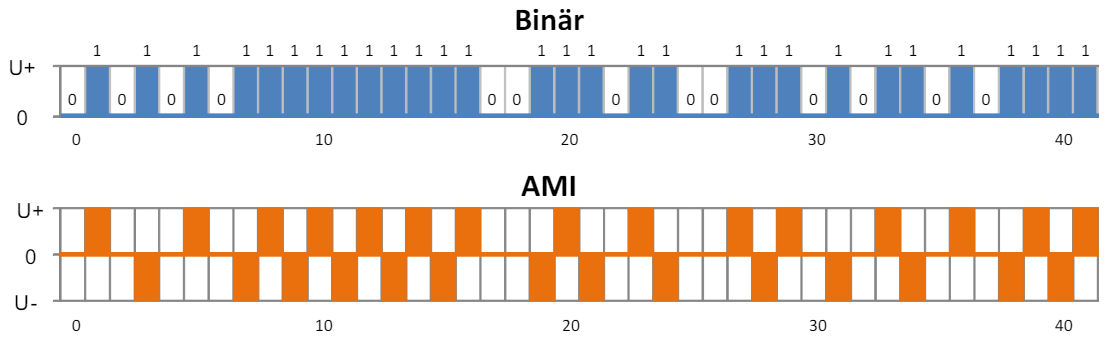
\includegraphics[width=0.8\linewidth]{images/gleichspannungsfreiheit.png}\\
    Nachteile dieses Leitungscodes:
    \begin{itemize}
        \item Auf der Übertragungsstrecke drei Zustände benötigt $\rightarrow$ rein binäre Medien genügen nicht
        \item Bei einer längeren Folge von 0 in den Daten ist keine Taktrückgewinnung mehr möglich
    \end{itemize}
\end{concept}

\begin{concept}{Manchester Leitungscode}\\
    wird z.B. bei 10BASE-T Ethernet verwendet, erlaubt einfache Taktrückgewinnung
    \begin{itemize}
        \item 1 positive Flanke, 0 negative Flanke
        \item Bei jedem Bit gibt es einen Signalwechsel
        \item Bandbreite von 10 MHz benötigt (2 $\times$ theoretisches Minimum)
    \end{itemize}
    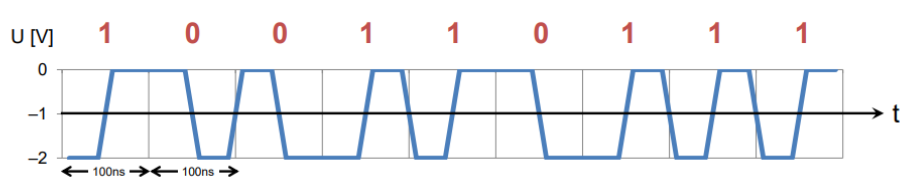
\includegraphics[width=0.6\linewidth]{images/leitungscode.png}
\end{concept}

\begin{concept}{NRZI MLT-3 Leitungscodierung}\\
    NRZI-Codierung (Non Return to Zero Inverted), kombiniert mit MLT-3\\
        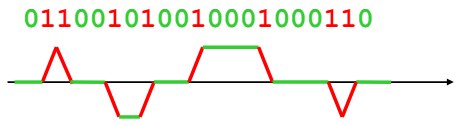
\includegraphics[width=0.5\linewidth]{images/leitungscodierung.png}\\
    MLT-3 = Multi-Level Transmit - Ternary
\end{concept}

\columnbreak

\subsubsection{Datenrate, Bandbreite, Bandrate}

\begin{formula}{Datenübertragungsrate}\\
    Die maximale Symbolrate $f_s$ (Baud) ist gleich der doppelten Bandbreite B (Hz) des
    Übertragungskanals. $$f_s = 2B$$
\end{formula}
\begin{example}
    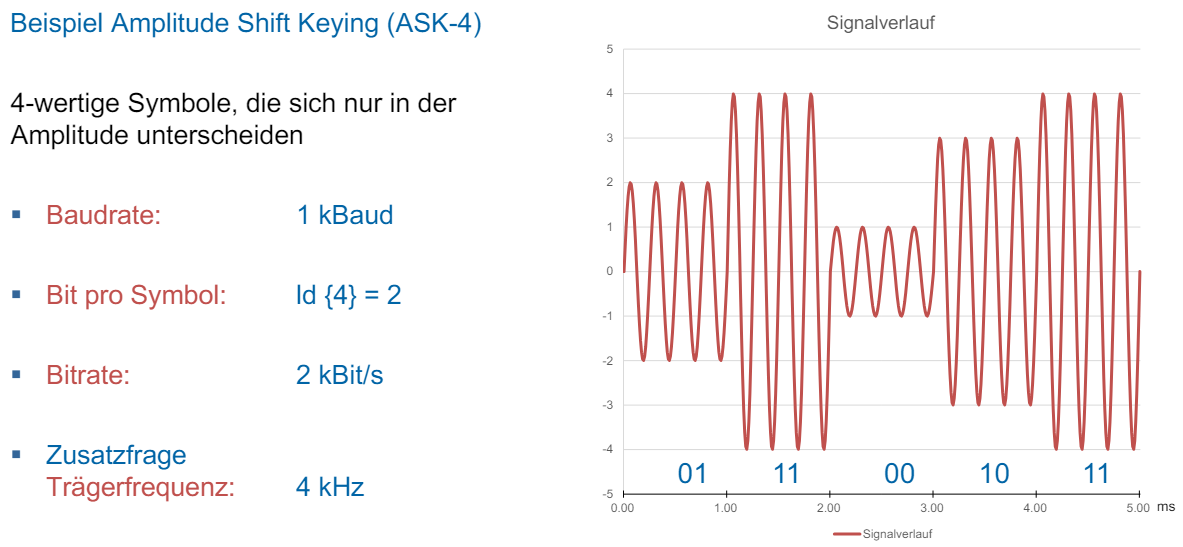
\includegraphics[width=1\linewidth]{images/amplitude_shift_keying.png}
\end{example}

\begin{formula}{Maximal erreichbare Bitrate}\\
    Maximale Bitrate $R[bit/s]$
    $$R \leq 2B \cdot log_2(M)$$
    Unterscheidbare Signalzustände
    $$M = 1 + \frac{A}{\Delta V}$$
    A = Max. Grösse des Signals\\
    V = Ungenauigkeit des Empfängers\\
\end{formula}
\centering
    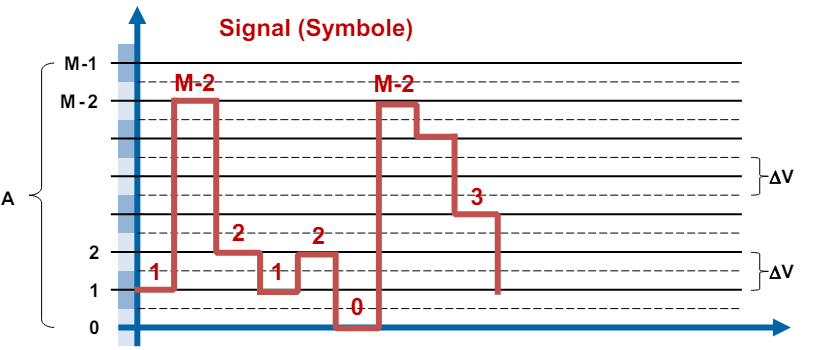
\includegraphics[width=1\linewidth]{images/max_bitrate_actual.png}

\begin{formula}{Kanalkapazität}
    $$C_s = B \cdot log_2(1 + \frac{S}{N})$$
    S: Signalleistung\\
    N: Rauschleistung
\end{formula}

\begin{KR}{Wichtige Kenngrössen}
    \begin{itemize}
        \item Bandbreite B – Einheit Hertz (Hz)
        \begin{itemize}
            \item Eigenschaft des Übertragungskanals und durch das Medium begrenzt
        \end{itemize}
        \item Symbolrate $f_s$ – Einheit Baud (Bd)
        \begin{itemize}
            \item Anzahl der Symbole pro Zeit. Limitiert durch die Bandbreite ($\leq$ 2B) (Nyquist)
        \end{itemize}
        \item Bitrate R – Einheit Bit/s (bps)
        \begin{itemize}
            \item Produkt von Symbolrate und mittlerem Informationsgehalt der Symbole (Hartley)
        \end{itemize}
        \item Kanalkapazität C – Einheit Bit/s (bps)
        \begin{itemize}
            \item Berücksichtigt für einen realen Kanal das Signal-zu-Rausch Leistungverhältnis S/N (Shannon)
        \end{itemize}
    \end{itemize}
\end{KR}

\begin{remark}
    \begin{itemize}
        \item In der Kommunikation stehen k, M, G etc. SI-konform für die exakten Zehnerpotenzen:
        \begin{itemize}
            \item kBit = $10^3$ Bit, MBit = $10^6$ Bit, GBit = $10^9$ Bit
        \end{itemize}
        \item Bitrate/Datenübertragungsrate/Durchsatz werden synonym verwendet
    \end{itemize}
\end{remark}

\begin{remark}
    ld = log2, lg = log10, ln = natürlicher Logarithmus
\end{remark}

\begin{KR}{Key Takes}
    \begin{itemize}
        \item Die physikalische Schicht befasst sich mit der Umwandlung physikalischer Signale (elektrisch, optisch) in einen Bitstrom und umgekehrt.
        \item Verkehrsbeziehung (Simplex/Duplex), Kopplung (Punkt-Pint oder Shared Medium) und Übertragungsverfahren (synchron/asynchron) sind bestimmende Eigenschaften.
        \item Die Leitungscodierung legt fest, wie genau diese Umsetzung erfolgt. Wichtige Anforderungen sind Gleichspannungsfreiheit und Taktrückgewinnung.
    \end{itemize}
\end{KR}
    \raggedcolumns
    %\newpage
    \section{Data Link Layer}
\paragraph{Schicht 2: Sicherungsschicht}

\begin{definition}{Framing (Rahmenbildung-/erkennung)}
    \begin{itemize}
        \item Senderichtung: Einpacken der zu sendenen Nutzdaten in Datenrahmen (Frames)
        \item Empfangsrichtung: Erkennung und Auspacken der Datenblöcke aus empfangenen Frames
    \end{itemize}
\end{definition}

\begin{concept}{Asynchron}
    {\small Keine Daten → Nichts gesendet (Pause zwischen Frames)}
    \begin{itemize}
        \item Zu Beginn eines Frames wird ein Start-Bit gesendet
        \item Prüfbits am Ende eines Frames!
        \item Frame-Grenze gibt auch Byte-Grenze
    \end{itemize}
\end{concept}

\begin{concept}{Synchron}
    {\small ohne Unterbruch $\rightarrow$ kontinuierlicher Bitstrom auf Phy. Layer}
    \begin{itemize}
        \item Stehen keine Daten an, werden Flags gesendet (anstatt Pause)
        \item Frames werden durch ein Start-Flag und ein End-Flag begrenzt:
    \end{itemize}
    \begin{minipage}{0.6\linewidth}
        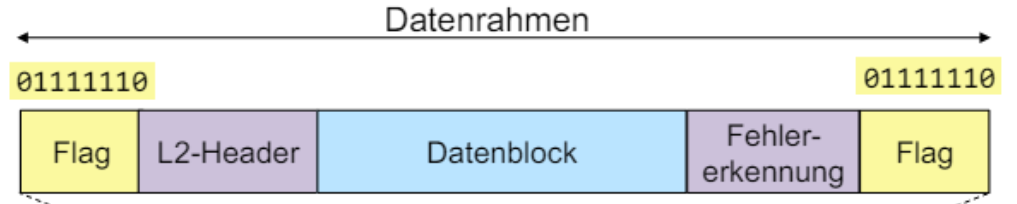
\includegraphics[width=1\linewidth]{images/images/flags_frames.png}
    \end{minipage}
    \begin{minipage}{0.39\linewidth}
        Maskierung von\\ Sonderzeichen (Flags)\\ nötig!
    \end{minipage}
\end{concept}

\begin{concept}{Bitstopfen} $\rightarrow$ um Bit-Muster zu garantieren 
    \begin{itemize}
        \item Sender fügt im Datenstrom nach 5 Einsen immer eine Null ein
        \item Empfänger wirft nach 5 Einsen immer ein Bit weg
        \item Somit gibt es (ausser bei Flags) nie die Bitfolge 01111110
    \end{itemize}
\end{concept}

\subsubsection{Framelänge und Fehlerwahrscheinlichkeit}

\begin{definition}{Fehlerwahrscheinlichkeit}
    \begin{itemize}
        \item BER (Bit Error Ratio) = 0.5 $\rightarrow$ jedes 2. Bit falsch
        \item FER (Frame Error Ratio): Fehlerhaft empfangene Frames
        \item RER (Residual Error Ratio): Unentdeckte fehlerhafte Frames
    \end{itemize}
\end{definition}

\begin{KR}{Frame-Fehlerwahrscheinlichkeit}

    Wahrscheinlichkeit dass Frame der Länge N min. 1 Bitfehler enthält:

    \vspace{0.5mm}

    $BER = p_e << 1 \longrightarrow (1 - p_e)^N \approx (1 - N \cdot p_e)$
    $$ \Rightarrow P_{Fehler, Frame} \approx N \cdot p_e (=FER)$$
\end{KR}

\begin{theorem}{Wahl der Framelänge} Overhead vs geringe Fehlerwahrscheinlichkeit
    \begin{itemize}
    \item Lange Frames:
    \begin{itemize}
        \item Höhere Nutzdatenrate ($\uparrow$ Netto-Bitrate, $\downarrow$ Overhead)
        \item $\Uparrow$ Fehlerwahrscheinlichkeit und Datenverlust pro Fehler 
        \item $\Uparrow$ Wahrscheinlichkeit eines unentdeckten Fehlers
    \end{itemize}
    \item Kurze Frames: Tiefere Nutzdatenrate, Zuverlässig
    \end{itemize}
\end{theorem}



\begin{formula}{Framelänge}
    Nettobitrate = Bruttobitrate $\cdot \frac{Nutzdaten}{Nutzdaten + Header}$
\end{formula}

\begin{formula}{Datenraten}  $F_R = \frac{B}{8\cdot(F_L + IFG)} \quad \quad \quad N = F_R \cdot P \cdot 8$ 
\end{formula}

\begin{remark}
    $F_R$ = Framerate, B = Bitrate, $F_L$ = Framelength, \\ IFG = Interframe Gap, N = Nutzbitrate, P = Payload
\end{remark}

\paragraph{Fehlererkennung und -korrektur}

\begin{concept}{Fehlererkennung} Redundanz $\rightarrow$ erhöht Hammingdistanz\\
    Zuverlässigkeit: abhängig von Framelänge/Verfahren
\end{concept}

\begin{remark}
    Standards IEEE 802 (LAN-Standards, zb Ethernet): 
    max. $5 \cdot 10^{-14}$ unentdeckte Fehler pro Frame-Byte,
    BER $p_e \leq 10^{-8}$ (1 Bitfehler pro 100 Mio. Bit)
    $\rightarrow$ CRC32 für Ethernet, mit Generatorpolynom (erkennt Fehler nur, korrigiert nicht)
\end{remark}

\begin{concept}{Fehlerkorrektur - Error Correction (EC)}
    \begin{itemize}
        \item Backward (BEC): erneutes Übertragen der Daten
        \item Forward (FEC): Rekonstruktion verfälschter Bits bei Empfänger
    \end{itemize}
\end{concept}

\begin{formula}{Hamming-Distanz} (h)
    \begin{itemize}
        \item Fehlererkennung: (h - 1) Fehler erkennbar
        \item Fehlerkorrektur: max. $\frac{h - 1}{2}$ Fehler korrigierbar
    \end{itemize}
\end{formula}

\begin{formula}{Einfache Parity}
    Prüfbit sichert ein Datenwort (typisch 1 Byte)\\
    Even Parity: Anzahl 1en inkl. Parity-Bit ist gerade (Odd analog)
\end{formula}

\begin{formula}{Längs- und Quer-Parity}\\
    3 Paritätsbits: 1 für jedes Byte, 1 für jedes Bit (Längs- und Quer-Parity), Gesamtparity

    \vspace{1mm}

    Korrigieren: 1 Bit-Fehler, Erkennen: 2 Bit-Fehler
\end{formula}


\subsubsection{Zugriffsmechanismen (Media Access)}

\paragraph{Gesteuerter Medium Zugriff}

\begin{definition}{Master-Slave Verfahren} Koordinierter Zugriff auf Medium
    \begin{itemize}
        \item Vorteil: Keine Konflikte, Master koordiniert Zugriff
        \item Nachteil: Ausfall des Masters (Single Point of Failure)
    \end{itemize}
\end{definition}

\begin{definition}{Token Verfahren} Sendeberechtigung in fixer Reihenfolge\\
    Knoten senden nur, wenn sie ein Token halten
    \begin{itemize}
        \item Vorteil:  Deterministisch (man weiss, wann man dran kommt)
        \item Nachteil: Aufwändiges Token Management (Startup, Token Verlust, etc.)
    \end{itemize}
\end{definition}

\begin{definition}{Zeitgesteuerter Zugriff} wie Taktfahrplan im Bahnnetz
    \begin{itemize}
        \item Vorteil: Optimierung möglich (nach Auslastung, Durchsatz, etc.)
        \item Nachteile: Planung und genaue Zeit in allen Knotepunkten erforderlich, Konflikte mit unplanbarem Verkehr
    \end{itemize}
\end{definition}

\paragraph{Random Medium Zugriff}

\begin{definition}{Carrier Sense Multiple Access} Vor Senden geteiltes Übertragungsmedium abhören ob frei (Carrier Sense), sonst bis Pause warten
    \begin{itemize}
        \item Vorteil: Alle Stationen gleichberechtigt (kein Master) \\ $\rightarrow$ jederzeit Zugriff auf Übertragungsmedium
        \item Nachteil: Kollisionen möglich (Collision Detection)
    \end{itemize}
\end{definition}

\begin{concept}{Kollisionsbehandlung - CSMA}
    \begin{itemize}
        \item CD (Collision Detection): Kollision: abbrechen, später nochmals
        \item CR (Collision Resolution): Hardware-unterstützte Arbitrierung
        \begin{itemize}
            \item Kollisionen werden erkannt und kontrolliert aufgelöst
        \end{itemize}
        \item CA (Collision Avoidance): Kollisionen vermeiden
        \begin{itemize}
            \item Request to Send / Clear to Send
        \end{itemize}
    \end{itemize}
\end{concept}

\begin{concept}{Flow-Control}\\
    Explizite Start-Stopp Signalisierung:
    \begin{itemize}
        \item Obere und untere Limite, stopp wenn oben, start wenn unten
    \end{itemize}
    Implizites Stop-and-Wait: Sender wartet auf ACK vor Senden
\end{concept}
    \raggedcolumns
    %\newpage
    \section{Ethernet und LAN}
\paragraph{Local Area Networks (LAN) Topologien}

    \centering
    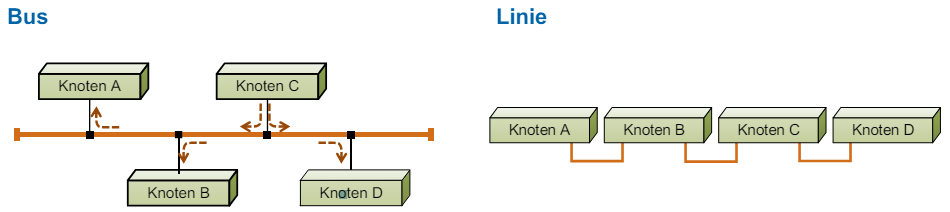
\includegraphics[width=0.85\linewidth]{images/images/bus_linie_topo.png}\\
    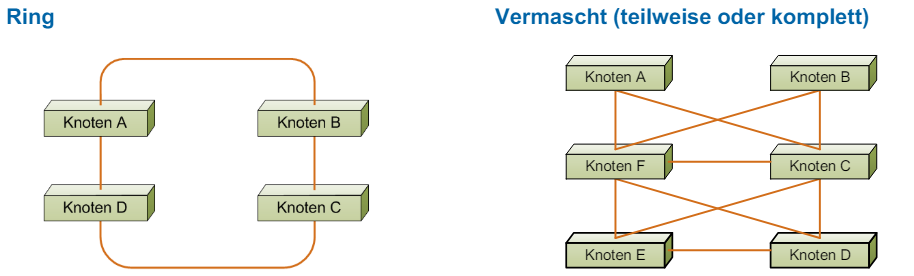
\includegraphics[width=0.85\linewidth]{images/images/ring_vermascht_topo.png}\\
    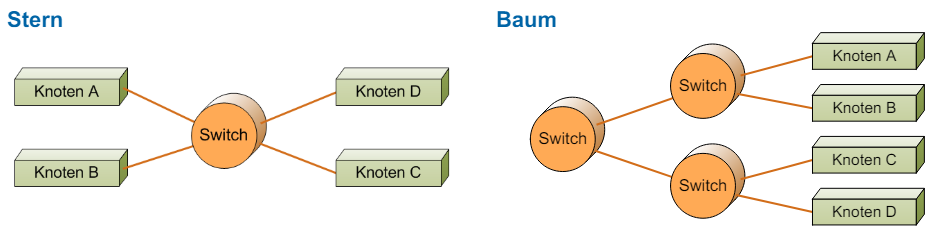
\includegraphics[width=0.85\linewidth]{images/images/stern_baum_topo.png}

\paragraph{Übertragung und Adressierung}

\begin{definition}{Übertragungsarten}
    Immer genau 1 Sender, E = \# Empfänger
    
    \begin{minipage}{0.35\linewidth}
        \includegraphics[width=0.4\linewidth, angle=90]{images/übertragungsarten.png}
    \end{minipage}
    \begin{minipage}{0.6\linewidth}
        \begin{itemize}
            \item Unicast: 1 E 
            \item Multicast: n E (Gruppe)
            \item Broadcast: alle Knoten im LAN
        \end{itemize}
    \end{minipage}
\end{definition}


\begin{formula}{IEEE MAC Adressen}
    \begin{itemize}
        \item 3-Byte «OUI» identifiziert Hersteller
        \item 3-Byte Laufnummer durch Hersteller verwaltet
    \end{itemize}
    \begin{minipage}{0.6\linewidth}
    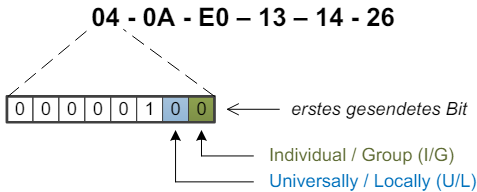
\includegraphics[width=1\linewidth]{images/images/klassifizierung_MAC_adresse.png}
    \end{minipage}
    \begin{minipage}{0.38\linewidth}
        Individual/Group Bit:
        \begin{itemize}
            \item 0 = individual address
            \item 1 = group address
        \end{itemize}
        Universally/Locally Bit:
        \begin{itemize}
            \item 0 = universally administrated adress
            \item 1 = locally administrated adress
        \end{itemize}
    \end{minipage}
\end{formula}

\begin{definition}{Ethernet Frame Format}\\
    \begin{minipage}{0.3\linewidth}
        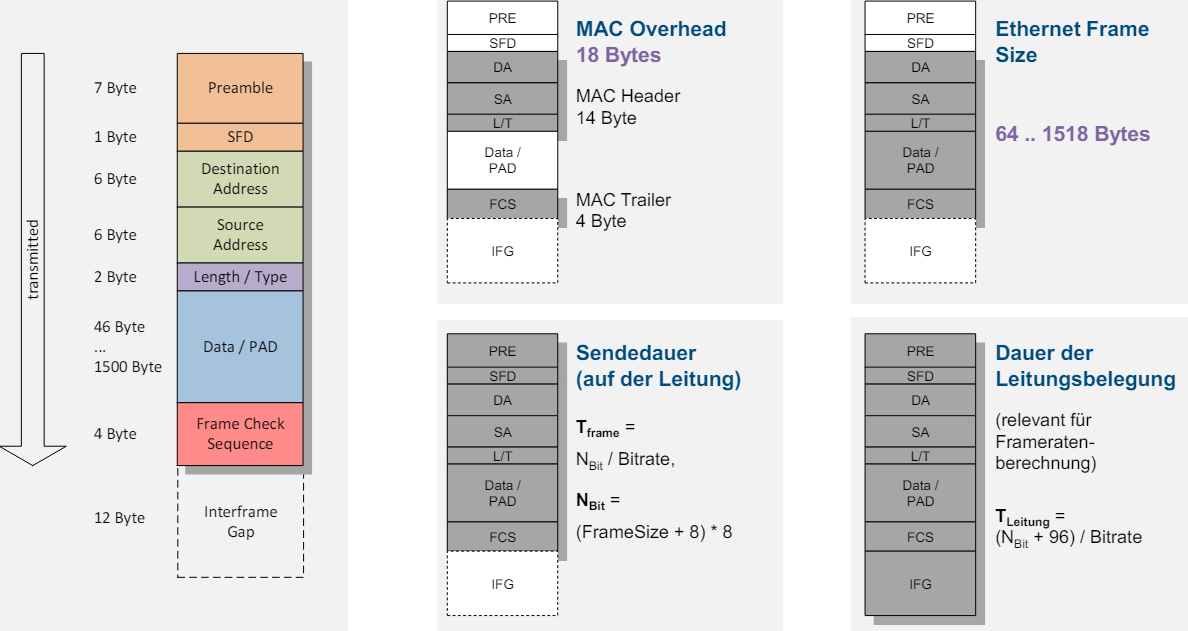
\includegraphics[width=0.9\linewidth]{images/images/ethernet_format.png}
    \end{minipage}
    \begin{minipage}{0.7\linewidth}
        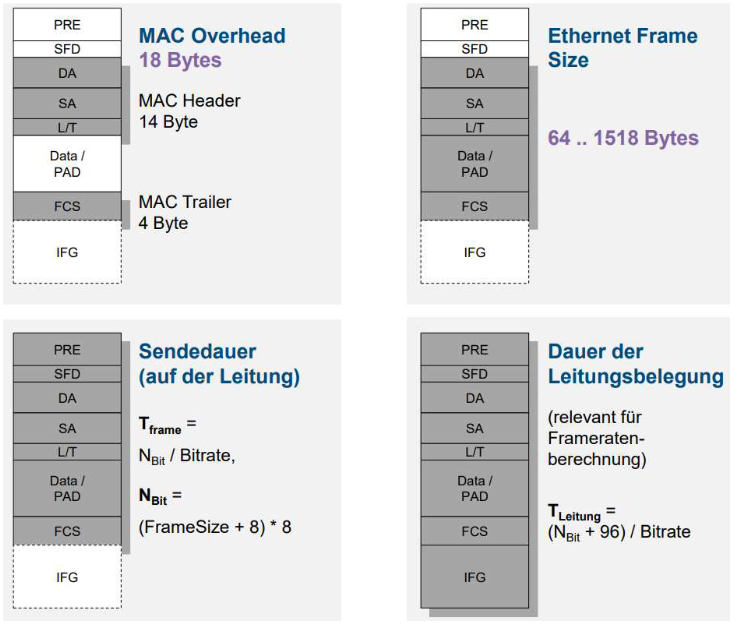
\includegraphics[width=1\linewidth]{images/images/ethernet_frame_details.png}
    \end{minipage}     
\end{definition}

\begin{theorem}{Bezeichnungsschema und Datenraten}\\
    \begin{minipage}{0.65\linewidth}
        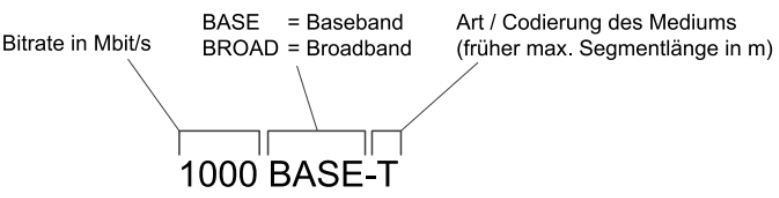
\includegraphics[width=1\linewidth]{images/images/ethernet_bezeichnungsschema.png}
    \end{minipage}
    \begin{minipage}{0.3\linewidth}
        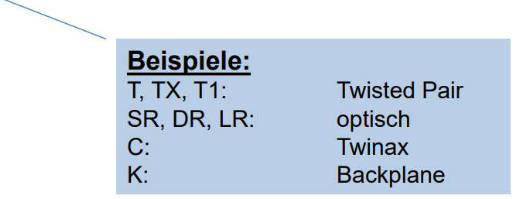
\includegraphics[width=1\linewidth]{images/images/ethernet_bsp_bezeichnung.png}
    \end{minipage}
\end{theorem}

\begin{example2}{Ethernet Frame Format und MAC-Adresse}\\
    Sende Ethernet-Frame über 100BASE-TX Schnittstelle\\ Bit-Sequenz auf Kabel:\\
    10101010 10101010 10101010 10101010 10101010 10101010\\
    10101010 10101011 00010000 00000000 01011010 11100011\\
    10011111 10000110 ...\\
    MAC-Adresse und Hersteller des Empfängers:
    \begin{itemize}
        \item 7 Bytes Präambel (10101010), 1 Byte SFD (10101011)
        \item 6 Bytes Destination Address: 00001000 (=08) 00000000 (=00) 01011010 (=5A) 11000111 (=C7) 11111001(=F9) 01100001(=61)
    \end{itemize}
    $\Rightarrow$ MAC-Adresse: 08-00-5A-C7-F9-61, Hersteller (08-00-5A) IBM
\end{example2}

\begin{remark}
    Pro Byte zuerst LSB, dann MSB (Ausnahme Zahlenwerte, z.B. Length/Type-Feld)
\end{remark}

\paragraph{Ethernet Geräte (Network Gear)}

\begin{definition}{Switch/Brigde} Signale weiterleiten und verstärken, zusätzlich:
    \begin{itemize}
        \item Prüft Checksumme und kann Layer-2 Adressen auswerten
        \item Transparent: sollen für Endgeräte unsichtbar sein
        \item Verwendet Filtering Database (Adress-Learning)
    \end{itemize}
\end{definition}

\begin{theorem}{Leistungserkmale von Switches und Bridges}\\
    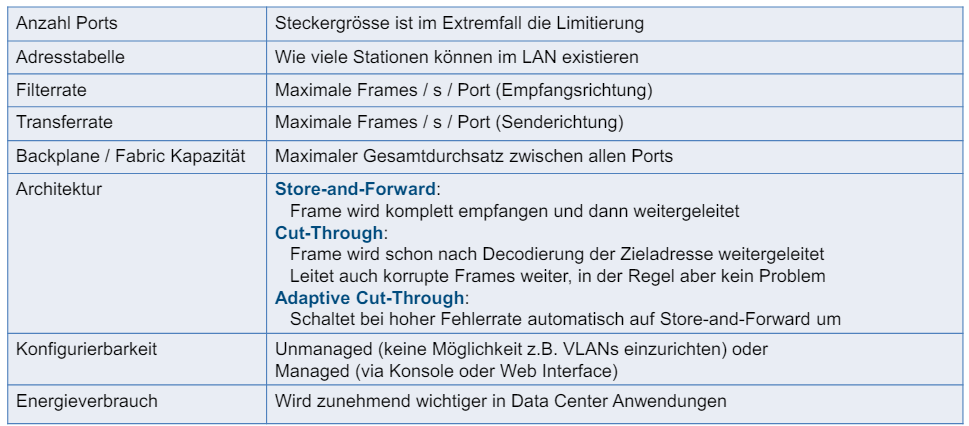
\includegraphics[width=1\linewidth]{images/images/merkmale_switches_bridges.png}
\end{theorem}


\begin{definition}{Filtering Database}\\
    Maps MAC-Adressen auf Ports (lernt nur Absenderadressen)\\
    Wenn Adresse bekannt $\rightarrow$ direkt an diese senden!\\
    Sonst: Flooding (Broadcast/Multicast)\\
    Vergisst Einträge nach gewisser Zeit (Aging Time)
\end{definition}

\begin{KR}{Weg/Zeit-Diagramm für das Senden eines Frames}\\
        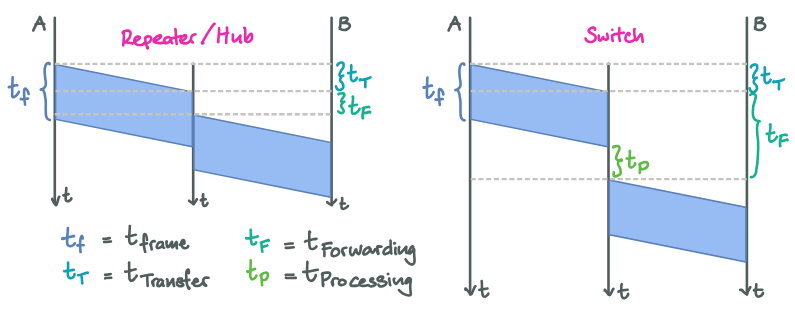
\includegraphics[width=1\linewidth]{images/images/zeit_frame.png}\\
        $t_f = \frac{F_L}{R}$ und $t_t = \frac{d}{C_{Medium}}$ $\Rightarrow$ Latenz $= t_f + t_t$
        
        \vspace{1mm}

        $t_F$ verlängern $\Rightarrow$ Verarbeitungszeit ermöglichen

        {\footnotesize $F_L$ = Frame Länge/Framesize, $R$ = Bitrate, $d$ = Distanz, $C_{Medium} 2/3 c_0$}
\end{KR}

\begin{formula}{Kollisionserkennung}
    Überlagerung von Signalen\\
        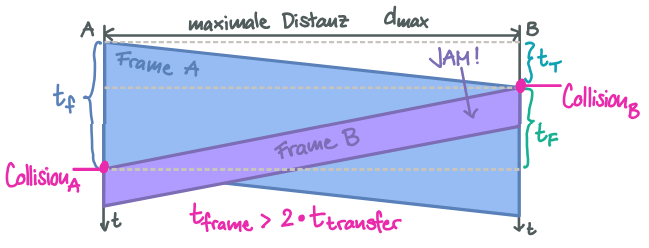
\includegraphics[width=0.8\linewidth]{images/images/frame_collision.png}\\
    Ein Knoten kann Kollisionen nur lokal erkennen, solange er selbst am Senden ist
    $$d_{max} < \frac{1}{2} \cdot \frac{Framesize_{min}}{Bitrate} \cdot C_{Medium}, d_{max} < \frac{1}{2} \cdot \frac{576 Bit}{10 \cdot 10^6 \cdot Bit/s}$$
\end{formula}

\begin{remark}
    Bedingung für Kollisionserkennung mit Repeater: $t_{frame} > 2 \cdot (\sum t_{transfer} + \sum t_{forwarding})$
\end{remark}

\paragraph{Redundanz (Spanning Tree)}

\begin{KR}{Spanning Tree Algorithmus}
    Redundante Pfade $\rightarrow$ Probleme! \\$\Rightarrow$ Ziel: Alle Segmente loop-frei verbinden

    \vspace{1mm}
    
        Initialisierung: Alle Ports für Nutzdaten blockiert, Annahme: «Ich bin Root», Austausch BPDUs mit Nachbarn (Root ID, Root Cost, Bridge ID, Port ID)
    
    \vspace{1mm}

    Aufbau des Spanning Tree: «kleinster» Nachbar als Root gesetzt \\ $\rightarrow$ Anzahl Hops + 1 (Beachte Prioritätswert)\\
    wiederholen bis alle dieselbe Root ID haben
    
    \vspace{1mm}

    \begin{minipage}{0.6\linewidth}
    Setzen der Port Roles: Root-Ports (Empfang der «besten» BPDU), Designated-Ports (Weg zum «kleinsten» Nachbar), Blockierte Ports (Discarding)
\end{minipage}
\hspace{1mm}
    \begin{minipage}{0.37\linewidth}
        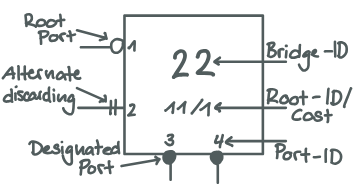
\includegraphics[width=1\linewidth]{images/images/spanning_tree_algorithmus.png}
    \end{minipage}
\end{KR}

\begin{example}
    \begin{minipage}{0.48\linewidth}
        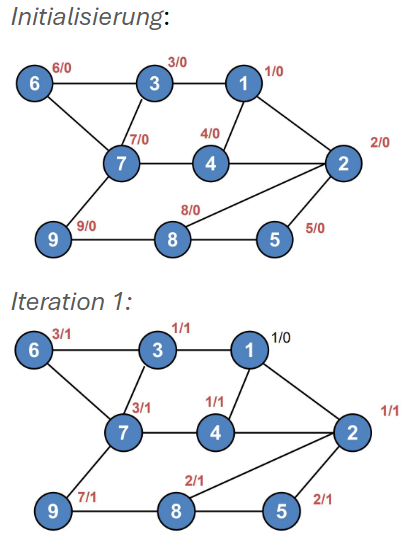
\includegraphics[width=0.8\linewidth]{images/images/rapid_spanning_tree1.png}
    \end{minipage}
    \begin{minipage}{0.48\linewidth}
        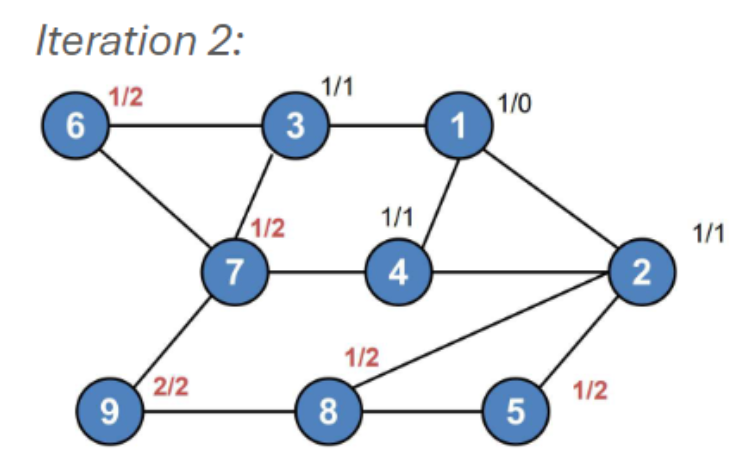
\includegraphics[width=0.8\linewidth]{images/images/rapid_spanning_tree2.png}\\
        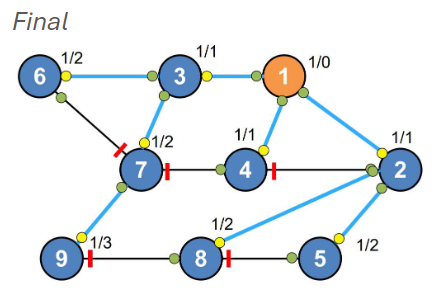
\includegraphics[width=0.8\linewidth]{images/images/rapid_spanning_tree3.png}
    \end{minipage}
\end{example}

\subsubsection{Virtuelle LANs}

\begin{definition}{VLAN}
    Aufteilen eines LANs in mehrere unabhängige logische Netze (Broadcast Domains)\\
    \begin{minipage}{0.65\linewidth}
        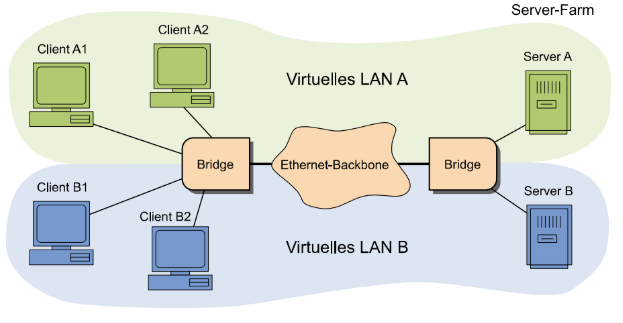
\includegraphics[width=1\linewidth]{images/images/vlan.png}
    \end{minipage}
    \begin{minipage}{0.3\linewidth}
        Trunk Links:
        Teil\\ mehrerer VLANs \\$\rightarrow$
        Frames eindeutig\\ kennzeichnen!
        \vspace{1mm}\\
        Trunk = Tagged\\ Access = Untagged
    \end{minipage}
\end{definition}

\begin{formula}{VLAN Tagging} Erweiterung Ethernet Header {\footnotesize (VLAN-Tag: +4 Bytes)}\\
    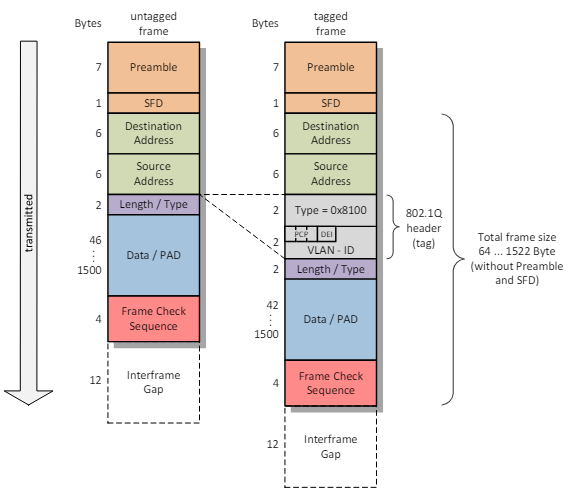
\includegraphics[width=1\linewidth]{images/images/vlan_tagging.png}
        \begin{itemize}
            \item VLAN-ID (VID) im VLAN-Tag: Zuordnung 
            \item Priority Code Point (PCP): ermöglicht Priorisierung
            \item Discard Eligibility Indicator (DEI) \\
            0 → Frame wird bei Überlastung zuerst verworfen
            \item Vorteile: Transparent für Endgeräte, VLAN Konfiguration nur im Netz (dh relativ simpel)
        \end{itemize}
\end{formula}


\begin{comment}
\begin{example}
    Gesendete Frames:
    \begin{center}
    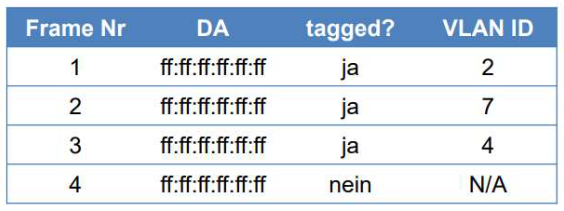
\includegraphics[width=0.5\linewidth]{images/images/bsp_vlan.png}
    \end{center}
    Switch Konfiguration:
    \begin{center}
    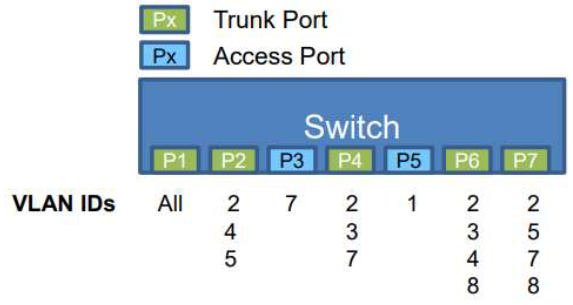
\includegraphics[width=0.5\linewidth]{images/images/vlan_example_switch.png}
    \end{center}
    Welche Frames werden an welchen Ports gesendet und sind diese getagged oder ungetagged?
    \begin{center}
    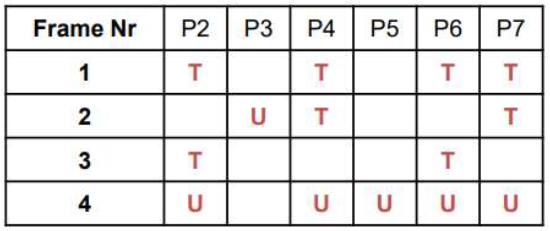
\includegraphics[width=0.5\linewidth]{images/images/vlan_example_frames.png}
    \end{center}
\end{example}
\end{comment}


\begin{example}
    \begin{minipage}{0.44\linewidth}
        Switch Konfiguration:\\
        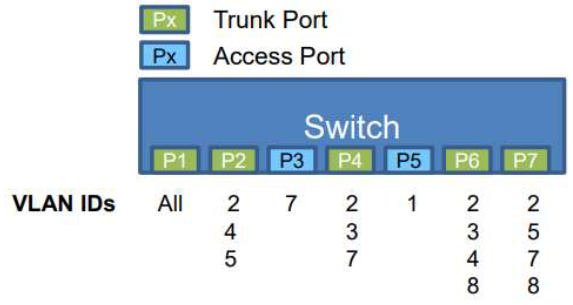
\includegraphics[width=1\linewidth]{images/images/vlan_example_switch.png}
    \end{minipage}
    \begin{minipage}{0.55\linewidth}
        Gesendete Frames:\\
        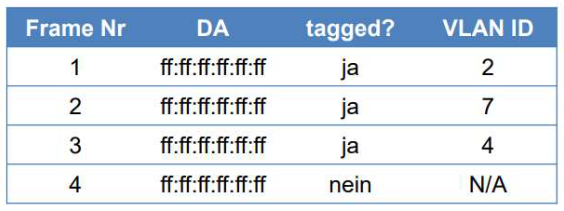
\includegraphics[width=1\linewidth]{images/images/bsp_vlan.png}
    \end{minipage}
    
    \begin{minipage}{0.4\linewidth}
        Welche Frames werden an welchen Ports gesendet und sind diese getagged oder \\ungetagged?
    \end{minipage}
    \hspace{5mm}
    \begin{minipage}{0.5\linewidth}
        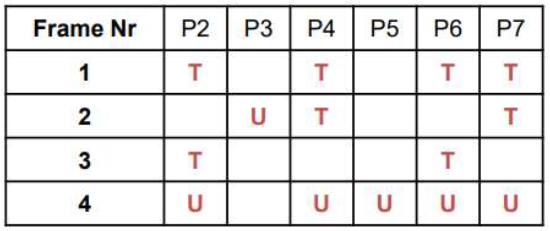
\includegraphics[width=1\linewidth]{images/images/vlan_example_frames.png}
    \end{minipage}    
\end{example}









    \raggedcolumns
    %\newpage
    \section{Network Layer}
\paragraph{Schicht 3: Internet}

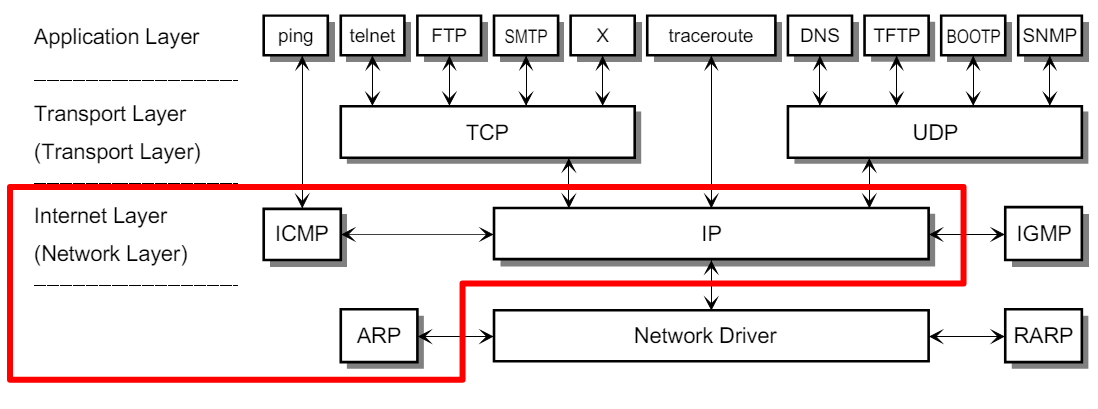
\includegraphics[width=1\linewidth]{images/orientierung_network_layer.png}

\begin{definition}{Die Netzwerkschicht}\\
    Verbindet Hosts in verschiedenen Netzen
    Transport der IP-Pakete $\rightarrow$ NUR Transport höhere Layer übernehmen:
        \begin{itemize}
            \item Fehlerfreie, komplette Übertragung
            \item Richtige Reihenfolge, Flusskontrolle
        \end{itemize}
\end{definition}

\begin{lemma}{Grundsätze des Internets}
    \begin{itemize}
        \item Jedes Netzwerk soll für sich selbst funktionsfähig sein
        \item Die Kommunikation basiert auf «best effort»
        \item Die Verbindung der Netze erfolgt durch Black Boxes
        \item Keine zentrale Funktionssteuerung wird benötigt
    \end{itemize}
\end{lemma}

\begin{definition}{Kommunikationsobjekte} OSI Layern zugeordnet
       \begin{itemize}
        \item \textcolor{orange}{(Application-)Message/Stream} Layer 5-7
        \item \textcolor{green}{(Transport-)Paket, Datagram} Layer 4
        \item \textcolor{blue}{(IP-)Paket (früher Datagram)} Layer 3
        \item \textcolor{pink}{(HW-specific) Frame} Layer 1-2
    \end{itemize}
\end{definition}



\subsection{Netzwerk Applikationen und Protokolle}

\subsubsection{Routing}

\begin{definition}{Router} verbinden Subnetze (Ethernet, xDSL, WLAN, etc.)
    \begin{itemize}
        \item empfangen nur Pakete, die direkt an sie adressiert sind
        \item Weiterleitung erfolgt anhand der Network Layer Adresse
        \item Benutzen immer den optimalen Pfad.
    \end{itemize}
\end{definition}
    

\begin{concept}{Routing and Forwarding}
    \begin{itemize}
        \item Routing: Aufbau und Update der Routingtabellen in den Knoten
            \begin{itemize}
                \item Router müssen optimalen Pfad zu jedem Host kennen
                \item kleine oder Teilnetze: Statische Konfiguration
                \item grössere Netze: Dynamisch durch Routing-Protokolle: Topologie des Netzes ermitteln $\rightarrow$ ideale Pfade bestimmen
            \end{itemize}
        \item Forwarding: Weiterleiten der Daten
        \begin{itemize}
            \item Aufgrund von Routingtabellen Datenpakete weiterleiten
        \end{itemize}
    \end{itemize}
\end{concept}

\begin{definition}{Routing-Tabelle} Info wie jedes Netz/Interface erreicht werden kann
    
    \begin{itemize}
        \item Für Weiterleitungsentscheidung notwendige Informationen:
        \begin{itemize}
            \item Eintrag für jedes erreichbare Netz (Netzadresse, Netzmaske)
            \item Interfaces, über die die Netze erreicht werden können
            \item IP-Adresse des nächsten Routers, wenn Zielnetz nicht direkt erreicht werden kann
        \end{itemize}
        \item Eigenschaften:
        \begin{itemize}
            \item sortiert nach Länge der Netzmaske, von oben nach unten durchsucht
            \item erster Eintrag der passt wird verwendet, default Eintrag am Schluss passt immer
        \end{itemize}        
    \end{itemize}
\end{definition}

\subsubsection{IPv4}

\begin{KR}{IP-Header Format}
    Ein IP-Packet besteht aus einem Header (min. 20 Byte) und Nutzdaten.
    \begin{itemize}
        \item \textcolor{blue}{Version} IPv4 / IPv6
        \item \textcolor{blue}{IHL} Header Length in 4-Byte (20 Byte → IHL = 5)
        \item \textcolor{blue}{Type of Service} neu Differentiated Services (DS), Erlaubt Priorisierung, Einteilung der Daten in Verkehrsklassen
        \begin{itemize}
            \item DSCP: spez. Verhalten bzgl. Weiterleitung
            \item ECN: kann drohende Überlast markieren
        \end{itemize}
        \item \textcolor{blue}{Total Length} Länge des IP-Packets (Header + Nutzdaten)
        \item \textcolor{Goldenrod}{ID Number} Identifikation des IP-Pakets / Fragmente, erlaubt Identifikation zusammengehöriger Fragmente
        \item \textcolor{Goldenrod}{Flags} Kontroll-Flags für Fragmentierung (0/DF/MF)
        \item \textcolor{Goldenrod}{Fragment Offset} Gibt an, wo ein Fragment hingehört
        \item \textcolor{green}{Time to Live} anz. Sek, Hop-Counter, 0 → Paket wird verworfen
        \item \textcolor{green}{Protocol} Übergeordnetes Protokoll
        \item \textcolor{purple}{Header Checksum} verhindert fehlgeleitete Pakete ($\times $ Nutzdaten)
        \item \textcolor{purple}{Source Address} Wer das Paket ursprünglich abgesendet hat
        \item \textcolor{purple}{Destination Address} Wer das Paket schliesslich erhalten soll
        \item \textcolor{purple}{Options/Padding} variabel, füllt auf ein Vielfaches von 32Bits auf
    \end{itemize}
        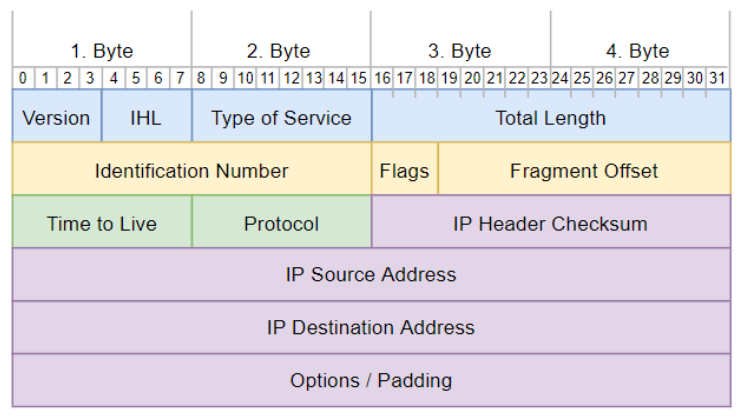
\includegraphics[width=1\linewidth]{images/internet_protokoll_format_ip.png}\\
    Das unterliegende Netz limitiert die Grösse eines Pakets (Maximum Transfer Unit). Der Sender kennt die MTU der Netze nicht.\\
\end{KR}

\subsubsection{Internet Protokolle (IP)}

\begin{definition}{Hierarchische Adressierung}\\
IP-Adressen sind zweistufig hierarchisch
\begin{itemize}
    \item IP-Adresse eines Hosts = Netzadresse + Interface-Adresse
\end{itemize}
\end{definition}

\begin{definition}{Terminologie}
    \begin{itemize}
        \item Sender und Empfänger $\rightarrow$ Hosts
        \item IP bietet einen unzuverlässigen, verbindungslosen Dienst
        \begin{itemize}
            \item IP-Adr. identifiziert Host-Interface (nicht den Host) eindeutig innerhalb des Netzwerks
            \item Jeder Host hat min. eine Adresse, Multi-Homed Hosts mehrere
        \end{itemize}
    \end{itemize}
\end{definition}

\begin{formula}{Netzadresse}
    \begin{itemize}
        \item Reserviert: Darf nicht für Interfaces verwendet werden!
        \item Tiefste Adresse im Subnetz (Interface-Adressbits alle 0)
        \item Berechnet durch: Interface-Adresse AND Subnetzmaske
    \end{itemize}
\end{formula}

\begin{formula}{Broadcast-Adresse}
    \begin{itemize}
        \item Reserviert: adressiert alle Interfaces in einem Subnetze
        \item Höchste Adresse im Subnetz (All Ones Broadcast)
        \item Berechnet durch: Interface-Adresse OR Invertierte Subnetzmaske
    \end{itemize}
\end{formula}

\begin{concept}{Subnetzmaske}\\
    bestimmt die Grenze zwischen Netz- und Interface-Adressbits:\\
        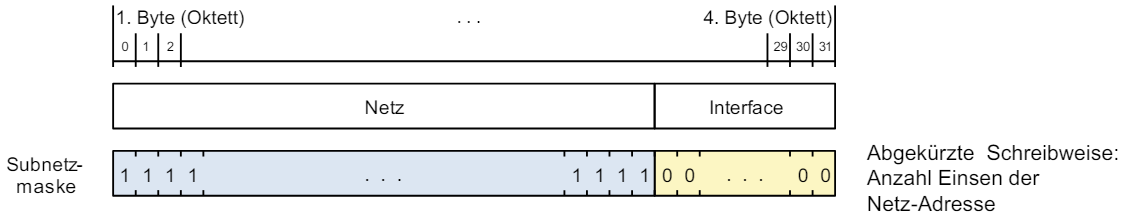
\includegraphics[width=1\linewidth]{images/subnetzmaske.png}\\
    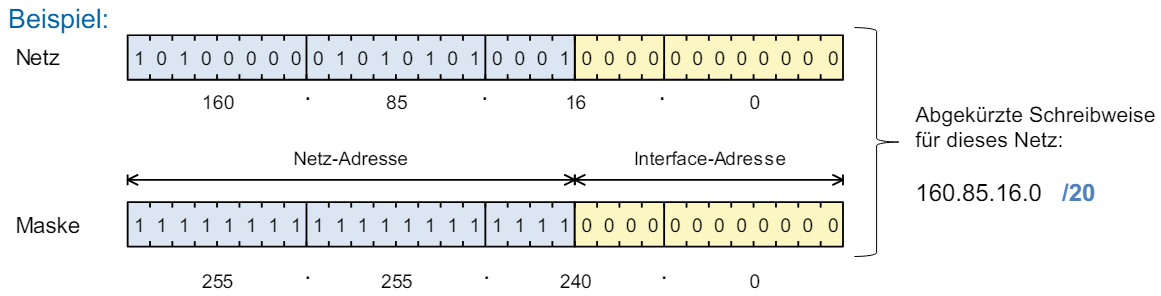
\includegraphics[width=1\linewidth]{images/subnetzmaske_bsp.png}   
\end{concept}

\begin{formula}{Netzmasken}\\
    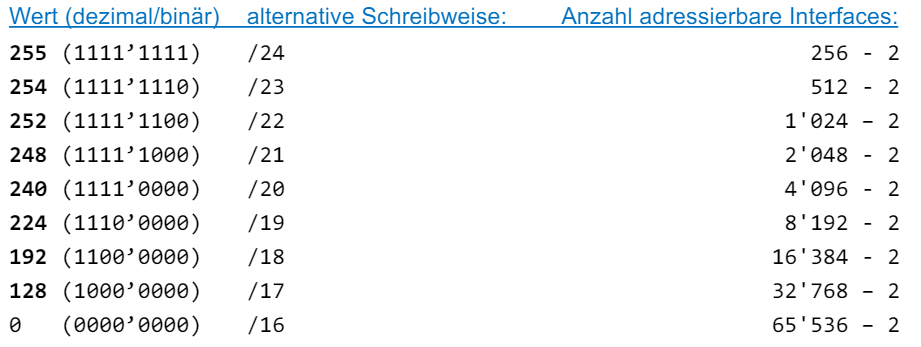
\includegraphics[width=1\linewidth]{images/subnetzmaske_bsp_2.png}
\end{formula}

\begin{KR}{Rechnen mit Netzmasken}\\
    Typische Internet-Adressen Aufgabenstellung: Berechnen Sie die fehlenden Informationen\\
        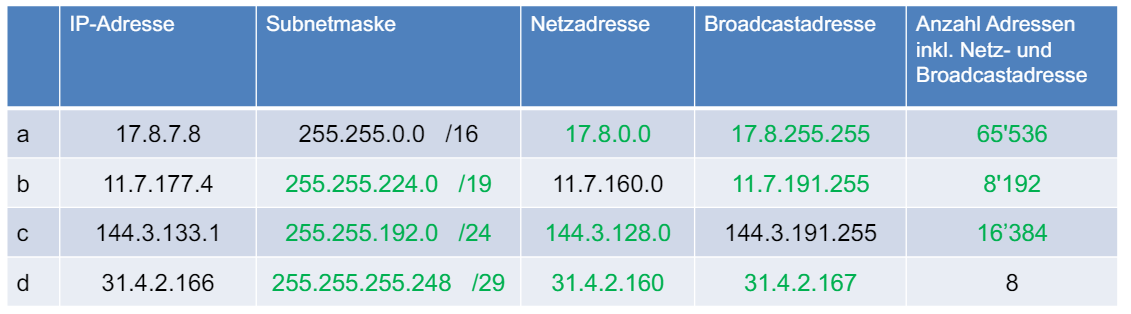
\includegraphics[width=1\linewidth]{images/rechenne_mit_netzmasken.png}

        Korrektur: Subnetzmaske c: /18 (nicht /24)
\end{KR}

\subsubsection{Flaches und Hierarchisches Routing}

\begin{concept}{Flaches Routing}
    \begin{itemize}
        \item Router kennt (evtl. mehrere) explizite Wege zu jedem Zielnetz
        \begin{itemize}
            \item Pakete an unbekannte Netze werden verworfen
        \end{itemize}
        \item Einsatz: stark vermaschte Netze oder zentraler Bereich (Backbone)
        \item Nachteil: Sehr grosse Routing-Tabellen
    \end{itemize}
\end{concept}

\begin{example2}{Flaches Routing Übung}
Was geschieht mit dem IP-Paket?
    \begin{itemize}
        \item Kein Unterbruch: Es wird nach gemäss dem 4. Eintrag der Routingtabelle von Router B an p0 weitergeleitet
        \item Unterbruch von p0/Router B: Es wird gemäss Eintrag 5 in der Routingtabelle von Router B an p2 weitergeleitet.
        \item zusätzlicher Unterbruch p0/Router C: Router C kann das IP-Paket nicht weiterleiten, es IP-Paket erreicht den Empfänger nicht.
    \end{itemize}
        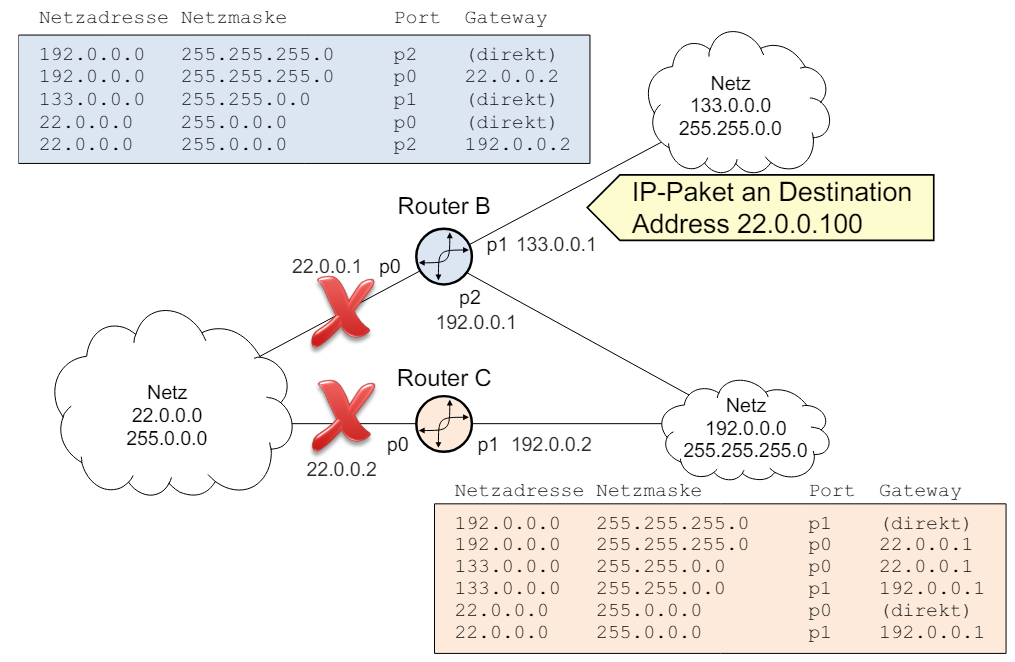
\includegraphics[width=1\linewidth]{images/flaches_routing_bsp.png}
\end{example2}

\begin{concept}{Hierarchisches Routing (Default)}
    \begin{itemize}
        \item Router kennt die direkt angeschlossenen Netze seiner Interfaces und genau einen anderen Router, an den er alles schickt, was für andere Netze bestimmt ist
        \begin{itemize}
            \item Der nächste Router geht genau gleich vor
        \end{itemize}
        \item Einsatz am „Rand“ von Netzen Hosts, ccess Router
        \item Kleine Routing-Tabellen mit jeweils einem Default-Eintrag
    \end{itemize}
        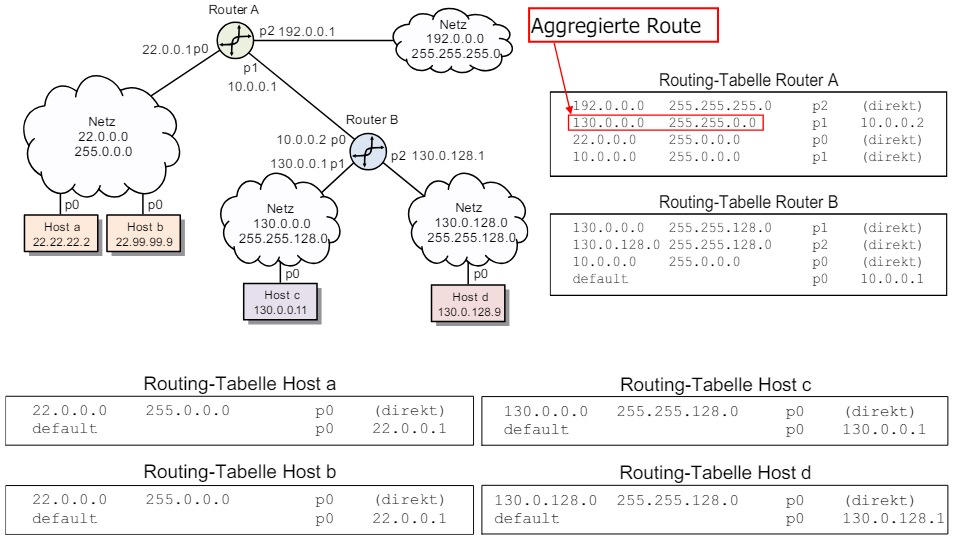
\includegraphics[width=1\linewidth]{images/hierarchisches_routing.png}
\end{concept}

\subsubsection{Classful Routing: Sub-/Supernetting}

\begin{concept}{Classful Routing}\\
    Ursprünglich war der IP Adressbereich in fünf Netzklassen (A - E) eingeteilt
    \begin{itemize}
        \item Eine Prefix (die ersten 4 Adress-Bits) erlaubt die Bestimmung der Klasse
    \end{itemize}
        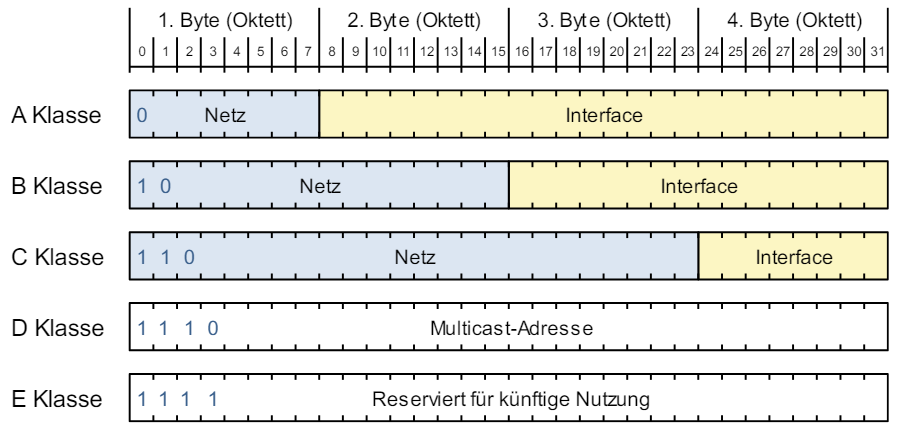
\includegraphics[width=0.9\linewidth]{images/classfulrouitng.png}
\end{concept}

\begin{KR}{Internet-Adressierung (IPv4 Netz-Klassen)}\\
    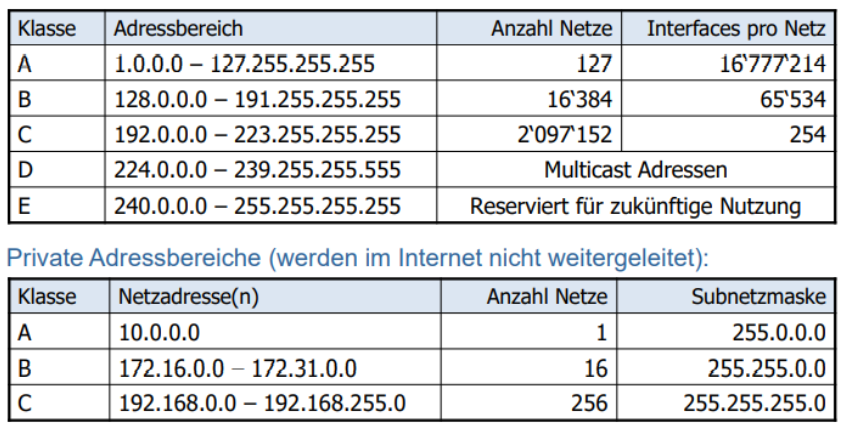
\includegraphics[width=0.8\linewidth]{images/ipv4.png}
\end{KR}

\begin{formula}{Adressbereiche für Classful Routing}
    \begin{itemize}
        \item klassische Netze fixer Grösse sind unflexibel (ungeeignet für Unternehmen)
        \\ $\rightarrow$ C zu klein, A zu gross, B zu wenig
        \item Abhilfe schafft CIDR – Classless Inter-Domain Routing
        \begin{itemize}
            \item Flexible Verwendung von Netzmasken beliebiger Länge
            \item Sub- und Supernetting
        \end{itemize}
    \end{itemize}
\end{formula}

\begin{definition}{localhost}
    Loopback-Adressen
    
    Das gesamte A-Netz 127.0.0.0/8 ist für Loopback-Test reserviert
\end{definition}



\paragraph*{Sub- und Supernetting}

\begin{concept}{Supernetting}
    Zusammenfügen von kleinen Netzen\\
    Hintereinanderliegende C Netze zu einem Netz zusammenfügen \\
    Bonus: Routingtabelle in Routern verkleinern (Aggregate Routes)
\end{concept}

\begin{example}
    Zusammenfassen von 4 Class C Netzen (22 = 2 Bits der Subnetzmaske)\\
        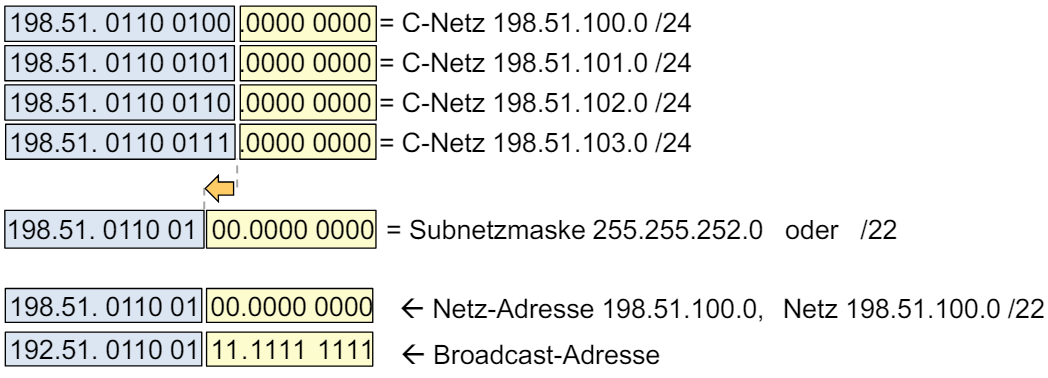
\includegraphics[width=1\linewidth]{images/example_supernetting.png}
\end{example}

\begin{concept}{Subnetting}
    Aufteilung in kleinere Netze\\
    ZHAW besitzt B Netz 160.85.0.0 $\rightarrow$ total $2^{16} \cong 65000$  Hosts
    \begin{itemize}
        \item in 8 kleinere Subnetze aufteilen → Subnetting
    \end{itemize}
    Verschieben der Netzmasken-Bits: 
    \begin{itemize}
        \item $8 = 2^3$, 3 Bits identifizieren 8 Subnetze (000 → 111) in binärer Netzmaske
        \item Netzmaske: /16 zu /19 (255.255.0.0 → 255.255.224.0)
        \item Interface-Anteil: $2^{16}$ zu $2^{13}$ = 8192 IP Adressen pro Subnetz
    \end{itemize}
        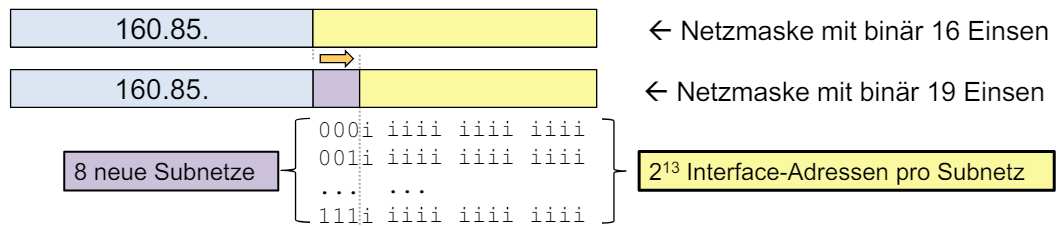
\includegraphics[width=1\linewidth]{images/subnetting1.png}\\
    Damit haben wir 8 neue Subnetze mit den folgenden Netzadressen:\\
        \includegraphics[width=0.75\linewidth]{images/subnetting2.png}
    \begin{itemize}
        \item Netz-Anteil: 19 statt 16 "1" → Subnetzmaske: 255.255.224.0 oder /19
        \item Host-Anteil: 13 statt 16 "0" → Anzahl Hostadressen = 8'192
    \end{itemize}
    Das zweite Netz oben wird deshalb korrekt wie folgt gekennzeichnet:
    \begin{itemize}
        \item 160.85.32.0 / 255.255.224.0 oder 160.85.32.0 /19
    \end{itemize}
    Das fünfte Netz wird wie folgt gekennzeichnet:
    \begin{itemize}
        \item 160.85.128.0 / 255.255.224.0 oder 160.85.128.0 /19
    \end{itemize}
    \textcolor{pink}{Wichtige Regel: Eine Netzwerkadresse ist immer ein Vielfaches der Netzgrösse!}
\end{concept}

\begin{example2}{Flexible Aufteilung eines Netzbereiches}\\
    4 Standorte, von ISP Netz 193.72.32.0 /21 erhalten. Ziel: 3 grössere und einen kleineren Standort redundant verbinden.\\
        \includegraphics[width=1\linewidth]{images/flexible_aufteilung_netzbereich.png}    
\end{example2}





\columnbreak

\subsubsection{Kapselung und Adressauflösung}

\begin{definition}{Kapselung eines IP-Pakets im Ethernet Frame} von Type 0x0806\\
        \includegraphics[width=1\linewidth]{images/kapselung_ip_paket.png}
\end{definition}



\paragraph*{Address Resolution Protocol (ARP)}

\begin{concept}{ARP}
    Ermittlung der Hardwareadresse (MAC) zu einer IP-Adresse
    \begin{itemize}
        \item ARP-Request wird an Broadcast-Adresse gesendet
        \item ARP-Response wird von Knoten mit angefragter IP-Adresse an Absender gesendet
    \end{itemize}
        \includegraphics[width=1\linewidth]{images/arp_concept.png}
\end{concept}

\begin{remark}
    Erkennung von Adresskonflikten: ARP Request an eigene IP-Adresse
\end{remark}

\begin{formula}{ARP Nachrichtenstruktur}\\
        \includegraphics[width=1\linewidth]{images/arp_nachrichtenstruktur.png}
\end{formula}

\begin{remark}
    Request: Destination Address = Broadcast, HW Address of Target = 0
\end{remark}

\begin{KR}{ARP Cache} mit bekannten HW-Adressen\\
    ARP für jedes IP-Paket ineffizient $\rightarrow$ Jeder Knoten führt ARP-Cache (speichert bekannte IP-MAC Kombinationen für gewisse Zeit)
\end{KR}

\begin{example}
    \includegraphics[width=1\linewidth]{images/encapsulation_bsp.png}\\
    \begin{itemize}
        \item a sendet IP-Paket c (Enthält Adressen a und c)
        \item a konsultiert Routing Tabelle $\rightarrow$ c kann über Router AB erreicht werden und a kennt nun IP-Adresse von Router AB
        \item a generiert Ethernet Frame, welches an HW-Adresse S von Router AB gesendet wird
        \begin{itemize}
            \item a muss aus IP-Adresse von Router AB die HW-Adresse S herausfinden $\rightarrow$ Adressauflösung
        \end{itemize}
        \item Router AB empfängt Ethernet Frame, packt IP-Paket aus und modifiziert den Header (TTL)
        \item Router AB konsultiert Routing Tabelle $\rightarrow$ c kann über Router BC erreicht werden und AB kennt nun IP-Adresse von BC
    \end{itemize}
    \textcolor{pink}{IP-Adressen a und c bleiben unverändert!}
\end{example}



\paragraph{Internet Control Message Protocol (ICMP)}

\begin{concept}{Internet Control Message Protocol (ICMP)}\\
    Übertragung von Fehlermeldungen oder Informationsaustausch
    \begin{itemize}
        \item nutzt direkt IP - keine Garantie, dass Meldungen ankommen
        \item Meldungen sind NUR informativ gedacht
    \end{itemize}
\end{concept}

\begin{KR}{ICMP Format}
    Header:
    \begin{itemize}
        \item \textcolor{blue}{Type} ICMP Typ
        \item \textcolor{green}{Code} Message Details
        \item \textcolor{green}{Checksum} Prüfsumme über die ICMP Meldung
        \item \textcolor{pink}{depends on code} Wert/Verwendung je nach ICMP Typ
    \end{itemize}
    \textcolor{purple}{Datenbereich} IP-Header und 64 Bits of Original Datagram
    \includegraphics[width=1\linewidth]{images/icmp_details.png}
\end{KR}

\begin{formula}{ICMP Meldungstypen}

    \begin{minipage}{0.5\linewidth}
        \begin{itemize}
            \item 0: Echo Reply
            \item 3: Destination Unreachable
            \item 5: Redirect
            \item 8: Echo Request
        \end{itemize}
    \end{minipage}
    \begin{minipage}{0.5\linewidth}
        \begin{itemize}
            \item 11: Time Exceeded
            \item 12: Parameter Problem
            \item 13: Timestamp Request
            \item 14: Timestamp Reply
        \end{itemize}
    \end{minipage}
\end{formula}

\begin{definition}{ICMP Destination Unreachable}
    Router/Zielhost $\rightarrow$ Absender\\ wenn Paket nicht weitergeleitet werden kann\\
        \includegraphics[width=1\linewidth]{images/destination_unreachable.png}
\end{definition}


\begin{KR}{Path MTU discovery} Vermeidung von Fragmentierung «unterwegs»\\
    Dazu: Erkennung der kleinsten MTU auf Pfad zwischen Sender und Empfänger (Path-MTU, PMTU)
    
    Vorgehen: (Annahme PMTU = lokale MTU)
    \begin{itemize}
        \item Sende IP-Pakete mit Länge=PMTU und mit DF=1
        \item Empfange «Destination Unreachable» mit Code 4 «fragmentation needed and DF set»
        \item PMTU reduzieren auf «Next-Hop MTU» (enthalten in Octet 5..8)
    \end{itemize}
\end{KR}

\begin{example2}{ICMP Destination Unreachable} Farben siehe IP-Header def.\\
    Host 160.85.31.3 sendet an Host 160.85.29.99:
    \begin{itemize}
        \item \textcolor{blue}{4500 0028} \textcolor{yellow}{8b10 0000} \textcolor{green}{0711} \textcolor{purple}{a8a4 \colorbox{lightgrey}{a055 1f03} \colorbox{lightgrey}{a055 1d63} 8b0d 829d 0014 a348 030a 0000 7504 1137 407c 0800}
        \item \colorbox{lightgrey}{Senderadr.}: a055 1f03, \colorbox{lightgrey}{Destinationadr.}: a055 1d63
    \end{itemize}
    Router kennt keinen Weg: sendet Destination Unreachable Message zurück:
    \begin{itemize}
        \item 4500 0038 8038 0000 fd\textbf{01} 5bc0 \colorbox{lightgrey}{a055 821e a055 1f03} \textcolor{blue}{03}\textcolor{green}{01 4bf7} \textcolor{pink}{0000 0000} \textcolor{purple}{4500 0028 8b10 0000 0711 a8a4 a055 1f03 a055 1d63 8b0d 829d 0014 a348}
        \item Erkennen dass dies ICMP Message ist: \textbf{Protocol}: 01
        \item ICMP Typ: \textcolor{blue}{Type}: 03
        \item 64 Bytes of Original Datagram: \textcolor{purple}{Original Data}
    \end{itemize}
\end{example2}














    \raggedcolumns
    %\newpage
    \section{Transport Layer}
\paragraph{Schicht 4: Transportschicht}

%\includegraphics[width=0.75\linewidth]{images/transportlayer.png}

\begin{definition}{Transportlayer}
    Schnittstelle zwischen Betriebssystem (Kernel Space) und Anwendungen (User Space)\\
    Zugriff auf Funktionen des Transport Layers erfolgt via klar definierten Schnittstelle (Sockets)
\end{definition}

\begin{definition}{Kapselung} "Protocol" Feld unterscheidet UDP und TCP Daten
    
    \includegraphics[width=0.9\linewidth]{images/tcp_udp_header.png}
\end{definition}

\begin{concept}{Adressierung}\\
    Client adressiert Server-Applikation mit Destination Port Nr.
    \begin{itemize}
        \item sonst weiss TCP/UDP-Modul im Empfänger nicht, welche Applikation gemeint ist
        \item für Source Port Nummer verwendet Client (meist) zufällige Port Nummer >1'023 (vom Betriebssystem vergeben)
    \end{itemize}
\end{concept}

\subsubsection{UDP - User Datagram Protocol}

\begin{definition}{UDP}
    Multi-/Demultiplexen der Datagramme zu Applikationen
    \begin{itemize}
        \item Verbindungslos und unzuverlässig
    \end{itemize}
\end{definition}

\begin{concept}{UDP-Header}
    \begin{itemize}
        \item \textcolor{green}{Source Port} Sendende Applikation
        \item \textcolor{green}{Destination Port} Applikation des Empfängers
        \item \textcolor{blue}{Message Length} Länge des Datagramms
        \item \textcolor{purple}{Checksum} Prüfsumme über einen Pseudo-Header, UDP-Header und Daten (kann Null sein)
        \begin{itemize}
            \item Pseudo-Header: IP Source- und Destination Address, Protocol Feld, Länge des Datagramms
            \begin{itemize}
                \item so können fehlgeleitete Datagramme erkannt werden
            \end{itemize}
        \end{itemize}
    \end{itemize}
        \includegraphics[width=0.9\linewidth]{images/udp.png}
\end{concept}

\begin{formula}{Port-Nummern}
    \begin{itemize}
        \item \textcolor{green}{System Ports (Well-Known)} Fix, für bekannte Appl. reserviert
        \item \textcolor{blue}{User Ports (Registered)} Reserviertert für herstellerspez. Appl.
        \item \textcolor{yellow}{Dynamic / Private Ports} Frei verfügbare Ports
    \end{itemize}
        \includegraphics[width=0.8\linewidth]{images/portnummern.png}
\end{formula}

\subsubsection{TCP - Transmission Control Protocol}

\begin{definition}{TCP Eigenschaften} 
    Verbindungsorientierte Übertragung, zuverlässiger Verbindungsaufbau, hohe Zuverlässigkeit, Vollduplexübertragung, Stream-Schnittstelle, Graceful Termination, Punkt-zu-Punkt Kommunikation
\end{definition}

\begin{concept}{TCP-Header Format}
    \begin{itemize}
        \item \textcolor{Goldenrod}{Sequence-Nr.} Sicherstellung Reihenfolge der Daten, Erkennung verlorener Daten
        \item \textcolor{Goldenrod}{Acknowledgement-Nr.} n + 1 $\rightarrow$ Daten bis und mit n korrekt und vollständig angekommen
        \item \textcolor{purple}{Data Offset} Gibt an wo Daten beginnen / enden
        \item \textcolor{purple}{ECN-Flags} Explicit Congestion Notification
        \begin{itemize}
            \item Bit 8: CWR (Congestion Window Reduced)
            \item Bit 9: ECE (ECN-Echo)
        \end{itemize}
        \item \textcolor{purple}{Control Bits} Verbindungsauf- und -abbau (Bits 10-15)\\
        URG: Urgent Pointer\\
        ACK: Acknowledgement Number (Bestätigung empfangener Daten, Erkennung verlorener Daten)\\
        PSH: Push (sofort ohne buffern weiterleiten)\\
        RST: Reset (Verbindung zurücksetzen oder geschlossenen Port signalisieren)\\
        SYN: Verbindungsaufbau,
        FIN: Verbindungsabbau
        \item \textcolor{blue}{Window} Verfügbare Puffergrösse 
        \item \textcolor{purple}{Urgent Pointer} URG = 1 $\rightarrow$ Position der wichtigen Daten
        \item \textcolor{purple}{Options} Häufigste Verwendung: MSS (Maximum Segment Size) die empfangen werden kann
    \end{itemize}
    \includegraphics[width=0.9\linewidth]{images/tcpheader.png}
\end{concept}

\paragraph{TCP Verkehrssteuerung}

\begin{concept}{Verbindungsorientierte Kommunikation}\\
    \includegraphics[width=1\linewidth]{images/zustandsdiagramm_tcp.png}
\end{concept}

\begin{KR}{Verbindungsaufbau und Verbindungsabbau}\\
\begin{minipage}{0.49\linewidth}
        \includegraphics[width=1\linewidth]{images/verbindungsaufbau.png}
\end{minipage}
\begin{minipage}{0.5\linewidth}
        \includegraphics[width=1\linewidth]{images/Verbindungsabbau.png}
\end{minipage}

ACK nr. muss mit der Anzahl der Bits der empfangenen Daten aktualisiert werden.
\end{KR}

\paragraph*{Vollständiges Beispiel}

\begin{example}
    Verbindungsaufbau:
    \begin{itemize}
        \item Server „horcht“ (LISTEN) auf einer bestimmten Port Nummer
        \item Client sendet Segment mit SYN=1 und zufälliger init. Sequenznummer a (ACK=0, weil ACK nr. ungültig)
        \item Server bestätigt Sequenznummer mit ACK nr. a+1 und ACK=1, wählt zufällige initiale Sequenznummer b, setzt SYN=1
        \item Client bestätigt b mit ACK nr. b+1 
        \begin{itemize}
            \item Erstes Byte vom Client zum Server hat Sequenznummer a+1
            \item Erstes Byte vom Server zum Client hat Sequenznummer b+1
        \end{itemize}
    \end{itemize}
        \includegraphics[width=1\linewidth]{images/example_verbindungsaufbau_tcp.png}
\end{example}

\begin{example}
    Datenaustausch: TCP-Nachrichten werden bi-direktional ausgetauscht\\
        \includegraphics[width=1\linewidth]{images/tcp_datenaustausch_ex.png}
\end{example}

\begin{example}
    Beide Seiten können den Verbindungsabbau einleiten
    \begin{itemize}
        \item Ist eine Richtung geschlossen (FIN, ACK), so können in die andere Richtung immer noch Daten gesendet werden (Half-Closed)
        \begin{itemize}
            \item In Richtung der "geschlossenen" Verbindung wird nicht mehr kommuniziert (Acknowledge number mismatch)
        \end{itemize}
        \item Falls die zweite Seite die Verbindung auch schliesst, können die 3. und die 4. Nachricht zusammengefasst werden $\rightarrow$ FIN/ACK
    \end{itemize}
        \includegraphics[width=1\linewidth]{images/tcp_verbindungsabbau_ex.png}
\end{example}





\subsubsection{TCP Adaptive Elemente}

\begin{formula}{Herausforderungen} zur Zuverlässigkeit zwischen Ethernet/TCP:\\
    \includegraphics[width=1\linewidth]{images/vergleich_layer_2_4.png}
\end{formula}

\paragraph*{Timed Delays}

\begin{formula}{Round Trip Time}
    dynamische Anpassung der Wartezeit 
    $$\alpha = 0.125: \textcolor{blue}{SRTT_n} = (1 - \alpha) \cdot \textcolor{blue}{SRTT_{n-1}} + \alpha \cdot \textcolor{green}{RTT_n}$$
    $$\beta = 0.25: \textcolor{Goldenrod}{RTTVAR_n} = (1 - \beta) \cdot \textcolor{Goldenrod}{RTTVAR_{n-1}} + \beta \cdot \textcolor{blue}{SRTT_n} - \textcolor{green}{RTT_n}|$$
    $$RTO_n = \textcolor{blue}{SRTT_n} + 4 \cdot \textcolor{Goldenrod}{RTTVAR_n}$$
\end{formula}

\begin{formula}{Bandwidth Delay Product (TCP-Puffergrössen)}\\
    \begin{minipage}{0.6\linewidth}
        Wahl der Grösse von Sende- und Empfangspuffer, um Verbindung nicht auszubremsen
        
        \resizebox{\linewidth}{!}{
        $BDP (bits) = RTT (sec) \cdot Bandbreite (bps)$}

        {\footnotesize RTT = Round-Trip-Time}
    \end{minipage}
    \begin{minipage}{0.35\linewidth}
        \includegraphics[width=1\linewidth]{images/bdp_rtt.png}    
    \end{minipage}
\end{formula}

\paragraph*{Fluss-Steuerung und Congestion Control}

\begin{concept}{Fluss-Steuerung}\\
        \includegraphics[width=1\linewidth]{images/fluss-steuerung.png}
\end{concept}





\begin{KR}{Sliding-Window TCP}
    \begin{itemize}
        \item Beide Richtungen arbeiten unabhängig voneinander
        \item Fenstergrösse wird in Anzahl Bytes angegeben
        \item Verbindungsaufbau: Initiale Fenstergrösse wird der anderen Seite mitgeteilt (Typische Werte: 16 / 32 / 64 KB)
        \item Pufferplatz im Empfänger wird alloziert
        \item Mit jedem ACK wird der verfügbare Pufferplatz (in Bytes) mitgeteilt und damit die Fenstergrösse dynamisch angepasst
        \item Fenstergrösse von 0 Bytes $\rightarrow$ keine Daten mehr senden
        \item Ist im Empfangsbuffer wieder Pufferplatz vorhanden, wird erneut eine Bestätigung mit diesem Pufferplatz an die andere Seite gesendet (= aktuelle Fenstergrösse)
    \end{itemize}
\end{KR}



\begin{example} Sliding Window TCP\\
        \includegraphics[width=1\linewidth]{images/flusssteuerung_tcp.png}\\
    Annahmen: 2'500 Byte Empfangspuffer, 5'000 Bytes Daten
    \begin{itemize}
        \item Fenstergrösse des Empfängers: WindowFeld des TCP-Headers
        \item Wireshark: Advertized Window Size
        \item Sender: nur einen Aufruf von send() für die gesamten 5'000 Bytes
    \end{itemize}
\end{example}

\begin{concept}{Congestion Control - Slow Start}\\
    \begin{minipage}{0.6\linewidth}
        \includegraphics[width=1\linewidth]{images/congestion_control.png}
    \end{minipage}
    \begin{minipage}{0.39\linewidth}
        {\small
        Slow Start: herantasten wie gross die einzelnen Frames sein können.

        \vspace{1mm}

        \textcolor{pink}{Wichtig:} Sender kombiniert Congestion Window mit\\ Informationen zur Flow\\ Control vom Empfänger\\ $\rightarrow$ schickt unbestätigte \\Daten bis min\{Congestion\\ Window, Advertised Win.\}\\ erreicht
        }
    \end{minipage}
\end{concept}


    \raggedcolumns
    %\newpage
    \section{Application Layer}

\subsubsection{Netzwerk-Applikationen und Protokolle}

\begin{KR}{Übersicht Applikationsprotokolle}
    \begin{itemize}
        \item Das Domain Name System (DNS) erlaubt übersetzt Hostnamen in IP Adressen und umgekehrt
        \begin{itemize}
            \item Besteht aus einem hierarchischen DNS Name Space
            \item Das DNS wird auf einer grossen Anzahl Name Server verteilt betrieben, ein Name Server ist jeweils für eine Zone verantwortlich (z.B. zhaw.ch)
        \end{itemize}
        \item DHCP erlaubt einem Rechner, seine IP Konfiguration von einem Server zu beziehen
        \item TFTP ist ein einfaches, aber zuverlässiges File Transfer Protocol, welches z.B. diskless Systemen dazu dient, das Betriebssystem Image vom Server zu beziehen
        \item HTTP erlaubt den Zugriff auf verteilte Dokumente, die mittels Uniform Resource Locator (URL) eindeutig adressiert werden
        \item Network Address Translation (NAT) erlaubt die Wiederverwendung privater IP-Adressen
    \end{itemize}
\end{KR}

\subsubsection{DNS - Domain Name System}

\begin{definition}{DNS - Domain Name Space}
    \begin{itemize}
        \item Leserliche Darstellung von IP-Adressen (Name Resolution)
        \item Hauptdomäne = Root
        \item Der Fully Qualified Domain Name (FQDN) muss eindeutig sein, Beispiel: sw.eng.
        \item Geschwisterknoten dürfen nicht den gleichen Namen haben
    \end{itemize}
    \includegraphics[width=1\linewidth]{images/dns_explained.png}
\end{definition}

\begin{concept}{Verwaltung von Domains}
    \begin{itemize}
        \item Das DNS wird verteilt betrieben (verteilt, nicht repliziert)
        \item Ein Name Server ist meist für eine Zone verantwortlich
        \begin{itemize}
            \item Zone: separat administrierter Subtree des DNS
            \item Ein Name Server kennt
            \begin{itemize}
                \item die IP-Adressen zu den Hostnamen in seiner Zone
                \item die IP-Adressen der Name Server seiner Subdomänen, falls diese nicht in seiner Zone liegen
                \item die IP-Adressen von Root und TLD Name Server, um beliebige Abfragen zu erlauben
            \end{itemize}
        \end{itemize}
        \item Aus Redundanzgründen min. zwei Name Server für eine Zone
        \begin{itemize}
            \item Primary (Master) und Secondary (Slave) 
        \end{itemize}
        \item Ein NS kann eine Unterzone seiner Zone weiter delegieren
    \end{itemize}
\end{concept}

\begin{definition}{DNS Record Types}\\
    Der "Record Type" enthält Information, welche Daten angefragt beziehungsweise in einer
    Antwort vom Name Server mitgeteilt werden\\
    \includegraphics[width=1\linewidth]{images/dns_record_types.png}
\end{definition}

\begin{definition}{Reverse DNS Lookup}\\
    Authentisierung: Ein Server identifiziert/authentifiziert einen Client anhand des Namens, nicht anhand der IP-Adresse
\end{definition}

\begin{example2}{DNS-Abfragen auswerten}
    \begin{itemize}
        \item DNS verwendet Port 53 (UDP)
        \item Resolver: lokale Software, die mit dem Name Server kommuniziert
    \end{itemize}
    Beispiel: Anwendung benötigt die IP-Adresse von bob.sw.eng.
    \begin{itemize}
        \item FQDN: bob.sw.eng. 
        \item Root: .
        \item Top Level Domain: eng
        \item Second Level Domain: sw
    \end{itemize}
        \includegraphics[width=1\linewidth]{images/example_dns.png}        
\end{example2}

\columnbreak

\subsubsection{NAT - Network Address Translation}

\begin{definition}{NAT (Port Mapping)}\\
    Alle Hosts im privaten Netz 192.168.0.0/8 verwenden 192.168.0.1 als Default-Gateway.\\
    Port-basierte NAT (NAPT) hat folgende Funktionen:
    \begin{itemize}
        \item Ersetzt private IP Adresse im IP Header durch eine öffentliche IP des Gateways / Routers
        \item Ersetzt die private Port-Nr. des Hosts durch eine freie zulässigen Port-Nr. des Gateways / Routers
        \item Erstellt ein Mapping von privater IP Adresse und Port-Nr. zur öffentlichen Port-Nr.
        \item Man kann für das Mapping auch statische Werte definieren, hier wird aber nur die Port-Nummer übernommen
    \end{itemize}
    Problem mit NAT:\\
    NAT verletzt das Konzept der OSI-Layer. Um einen Port im TCP Header zu ändern muss man eigentlich die
    Daten im IP-Frame ändern. Bedeutet eine Netzwerk-Funktion greift auf den Transport Header zu.
    IP-Adresse und Portnummer werden dabei verändert. \\
        \includegraphics[width=1\linewidth]{images/NAT.png}
\end{definition}

\columnbreak

\subsection{DHCP - Dynamic Host Configuration Protocol}

\begin{definition}{Bezug IP-Adresse}\\
    Wie erhält ein Knoten seine IP-Adresse?
    \begin{itemize}
        \item Lokal konfiguriert (static IP)
        \item Bezug der IP-Adresse über das Netzwerk
        \begin{itemize}
            \item DHCP – erlaubt dynamische Zuteilung aus dem lokalen Adressbereich
        \end{itemize}
    \end{itemize}
\end{definition}

\begin{concept}{Dynamische Zuweisung von IP-Adressen}
    \begin{itemize}
        \item Client verlangt eine IP-Adresse (DHCP Request)
        \item DHCP-Server erteilt eine freie Adresse für definierte Lease Time, oft 10 Minuten (DHCP-Response)
        \item Vor Ablauf der Lease Time muss der Lease (vom Client) erneuert werden
        \item Client, der das Netz verlässt, wird Lease nicht erneuern $\rightarrow$ Adresse wieder frei
    \end{itemize}
\end{concept}



\begin{KR}{Ablauf DHCP}
    \begin{enumerate}
        \item Client sucht DHCP Server mittels Broadcast
        \item DHCP Server antwortet (DHCP offer)
        \item Der Client wählt einen Server und fordert eine Auswahl der angebotenen Parameter (DHCP request)
        \item Der Server bestätigt mit einer Message, welche die endgültigen Parameter enthält
        \item Vor Ablauf der Lease-Time erneuert der Client die Adresse.
    \end{enumerate}
\end{KR}

\columnbreak

\begin{definition}{DHCP - Dynamic Host Configuration Protocol}
    \begin{itemize}
        \item Dynamische Zuweisung von IP-Adressen
        \item Reserviert nur IP’s von aktiven Geräte
    \end{itemize}
    \includegraphics[width=1\linewidth]{images/bootp.png}
\end{definition}

\begin{definition}{DHCP Paketformat}\\
    \includegraphics[width=1\linewidth]{images/dhcp_format1.png}\\
    \includegraphics[width=1\linewidth]{images/dhcp_format2.png}
\end{definition}







    \raggedcolumns
    %\section{Beispiele}

\subsection*{Übertragungsmedien}

\begin{example2}{Bandbreite von Twisted-Pair Kabeln}

Bei allen TP Kabelkategorien steigt der Dämpfungsbelag mit zunehmender Frequenz beinahe gleich an

Was ist der Grund, dass CAT5 Kabel mit einer Bandbreite von100 MHz verwendet werden, während CAT7 Kabel bis zu 600 MHz eingesetzt werden?

\emph{Antwort:}
Die Dämpfung ist nicht die einzige Grösse, welche die effektiv nutzbare Bandbreite eines Kabels bestimmt. Höherwertige Kabel habe eine viel besseres Übersprechverhalten, so dass eine höhere Dämpfung akzeptiert werden kann.
\end{example2}

\begin{example2}{Optische Übertragungsmedien}\\
  Die optische Sendeeinrichtung sendet mit $10^{-3}$ Watt Leistung. Für eine genügende Übertragungsqualität muss
  der Leistungspegel beim Empfänger mindestens $10^{-5}$ Watt betragen. Der Lichtwellenleiter hat einen
  Dämpfungsbelag von $0.5 \mathrm{~dB} / \mathrm{km}$. Welche Distanz kann überbrückt werden?

 \textbf{Antwort:}
Die erlaubte Abschwächung der Leistung entspricht dem Faktor 100, also $20 \mathrm{~dB}$. Demzufolge darf die Leitung maximal $40 \mathrm{~km}$ lang sein.
\end{example2}

\subsection*{OSI Modell}

\begin{example2}{Klassifizierung von Diensten}
  Zwei Schichten M und N haben zur jeweils höheren Schicht die folgenden Interfaces. Klassifizierung der Dienste?

  \vspace{1mm}

  M:

connect\_M (dest\_addr, options, \&handle)\\
send\_M (handle, options, numBytes, \&data)\\
..\\
close\_M (handle)

\emph{Antwort:} verbindungsorientiert, Connect/Close der Verbindung

\vspace{1mm}

N:

send\_telegramm\_N (remote\_addr, numBytes, \&data)\\
receive\_telegram\_N (\&remote\_addr, \&local\_address, \&buffer, bufsiz)

\emph{Antwort:} verbindungslos, keine Funktion zum Auf-/Abbau einer Verb.
\end{example2}

\subsection*{Physical Layer}

\begin{example}
    \includegraphics[width=1\linewidth]{images/images/amplitude_shift_keying.png}
\end{example}

\begin{example2}{Maximale Bitrate}
  Ein Übertragungssystem nutzt eine Bandbreite von $100 \mathrm{MHz}$ und codiert den Bitstrom mit 4wertigen Symbolen.
 
  Welches ist die theoretisch erreichbare maximale Bitrate?
 
 \textbf{Antwort:}
 $max_{Symbolrate} =200 \mathrm{MBd}$\\
 2 Bit/Symbol $\rightarrow$ $max_{Bitrate}$ $=400 \mathrm{Mbit} / \mathrm{s}$
 
 \vspace{2mm}
 
 Zur Steigerung der Bitrate wird ein 8-wertiger Code in Erwägung gezogen. Unter welchen Voraussetzungen ist das möglich?
 
 \textbf{Antwort:}
 Der Signal/Rauschabstand S/N muss genügend gross sein. Das ergibt sich aus der Sendeleistung, der Leitungsdämpfung und der Störleistung
 \end{example2}


 \begin{example2}{Maximale Zeichenrate}
 Wir betrachten eine asynchrone Schnittstelle, welche mit folgenden Parametern betrieben wird: Bitdauer T ist $1 \mathrm{~ms}$, 8 Bit/Zeichen, 1 Stopp-Bit.
 
 a) Welche maximale Zeichenrate lässt die Schnittstelle zu?
 
 \textbf{Antwort:}
 1000 Bit/s / 10 Bit/Zeichen = 100 Zeichen/s
 
 b) Um wieviel darf die Frequenz des Empfängertaktgebers von dem des Senders maximal abweichen, ohne dass das einen Übertragungsfehler bewirkt? Relative Angabe in Prozent.
 
 \textbf{Antwort:}
 Zeitmessung startet mit der fallenden Flanke des Start-Bits nach 9.5*T ist man im Idealfall in der Mitte des letzten Datenbits,
 Fehlablesung entsteht dann, wenn man um 0.5*T daneben liegt $\rightarrow 0.5 * \mathrm{~T} / 9.5 * \mathrm{~T}=1 / 19=5.26 \%$

 c) Wir betrachten den Fall, bei dem die Frequenz des Empfängertaktgebers geringfügig höher ist, als der unter b) errechnete Wert. Es wird das Zeichen 10101010 gesendet. Welches Zeichen detektiert der Empfänger?

 \textbf{Antwort:}
Das zuletzt übertragene Bit wird nicht abgetastet, dafür das vorhergehende zweimal. Weil das letzte Bit das MSB ist, wird das Zeichen 00101010 empfangen.
 \end{example2}



 \begin{example2}{Codierung auf Leitungen}

  a) Welche Eigenschaft muss ein Leitungscode aufweisen, dass der Empfänger den Takt aus dem Datenstrom extrahieren kann?
  
  \textbf{Antwort:} Der Bitstrom muss so codiert werden, dass er - unabhängig von den übertragenen Daten - genügend häufige Pegeländerungen (Signalflanken) aufweist.
  
  b) Nennen Sie zwei Codes, welche die Bedingung unter a) erfüllen.
  
  \textbf{Antwort:} Manchester (10Base2, 10BASE-T), dreiwertiger NRZI mit 4B5B Codierung (100Base-TX), 4B3T (10BASE-T1L)
  
  c) Aus welchen Gründen kann es notwendig sein, dass ein Leitungscode gleichstromfrei ist? 
  
  \textbf{Antwort:} Wird das Signal galvanisch getrennt über einen Transformator geführt wird, dann geht der Gleichstromanteil verloren.
  
  d) Nennen Sie zwei Codes, welche gleichstromfrei sind. \textbf{Antwort:} AMI, 4B3T (10BASE-T1L), dreiwertiger NRZI (100Base-T)
 \end{example2}

 \begin{example2}{Ein Übertragungsverfahren}
  soll 320 MBit/s übertragen können. Die im Übertragungsmedium nutzbare Bandbreite $B$ beträgt $40 \mathrm{MHz}$.

Wie viele Zustände pro Symbol muss das Codierungsverfahren bieten, damit bei maximaler Symbolrate die geforderte Bitrate erreicht werden kann? 

\textbf{Antwort:}
Hartley: Bitrate $=2$ * $B$ * $\operatorname{Id}(\mathrm{N})$

$\rightarrow 320 \mathrm{Mb} / \mathrm{s}<=80 \mathrm{MHz}$ * Id $(\mathrm{A})$

$\rightarrow \operatorname{Id}(A)>=4$ Damit werden mindestens $2 * * 4=16$ Zustände benötigt.
 \end{example2}

\subsection*{Data Link Layer}

\begin{example2}{Datenübertragung und Framing}\\
    Gegeben: Bitrate 100 Mbit/s, Frame-Länge 1000 Byte, IFG 96 Bit, Payload 800 Byte. Berechnen Sie die Nutzdatenrate.\\
    \textbf{Lösung:}\\
    $$F_R = \frac{100 \cdot 10^6}{8 \cdot (1000 + 96)} = 1.19 \cdot 10^6 \text{ Frames/s}$$
    $$N = 1.19 \cdot 10^6 \cdot 800 \cdot 8 = 7.6 \cdot 10^9 \text{ Bit/s} = 7.6 \text{ Gbit/s}$$
\end{example2}

 \begin{example2}{Bitstuffing}
  Synchrone Datenübertragung und Codes
  
  Bei der synchronen Datenübertragung werde das Flag 01111110 und Bit-Stuffing (Bitstopfen) verwendet.
  
  a) Wozu verwendet man hier Bit-Stuffing?
  
  \textbf{Antwort:}
  Start-/Ende-Flags dürfen nicht in den eigentlichen Daten vorkommen, da dies vom Empfänger als Flag detektiert würde
  
  b) Wie sieht der folgende gesendete Bitstrom auf der Leitung aus?
  
  \textbf{Antwort:}

  1010111111010011111111111000000101011111011111101
  
  10101111\textbf{0}1010011111\textbf{0}11111\textbf{0}11000000101011111\textbf{0}011111\textbf{0}101
  \end{example2}

  \begin{example2}
    {Fehlerkorrektur beim Stop-and-Wait Protokoll}

  Der Sender erkennt durch einen Timeout eine fehlende Bestätigung und wiederholt daraufhin das zuletzt gesendete Telegramm.
  \end{example2}

\subsection*{LAN und Ethernet}

\begin{formula}{GBASE-T}\\
    \includegraphics[width=1\linewidth]{images/images/GBASE-T.png}
\end{formula}

\begin{example2}{100Base-TX Kabel und Stecker}

  Charakterisieren Sie das für 100 Base-TX verwendete Kabel (inkl. Stecker). Worin können sich solche Kabel unterscheiden?

- UTP (Kabel, das ungeschirmte verdrillte Aderpaare enthält). Das universell verwendbare Kabel enthält 8 Adern, von denen bei 100 Base-TX nur 4 verwendet werden.

- Üblicher Stecker ist vom Typ RJ45.

- Unterschiede: Es gibt 1:1 und Crossover - Kabel. Die Übertragungseigenschaften können sehr verschieden sein und werden durch die Kabelkategorie charakterisiert.
\end{example2}

\begin{example2}{100Base-TX Oszilloskop}\\
 Sie sehen auf einem Oszilloskop das folgende Bild eines 100Base-TX Signals:
  \begin{center}
  \includegraphics[width=0.8\linewidth]{images/images/2024-06-20-17-47-36.png}
  \end{center}
Ein Kästchen entspricht einem Bit. Wie lauten die ersten 10 Bits?

\textbf{Antwort:}
1100010101
\end{example2}


\begin{example2}{Ethernet Segment Rate}
Wie viele Frames pro Sekunde können auf einem 100 Base-TX Ethernet Segment pro Richtung maximal übertragen werden?
Hinweis: Denke an Inter-Frame Gap, die mindestens so lange wie die Übertragung von 12 Bytes dauert.

\textbf{Antwort:}
Die grösste Frame Rate wird erreicht, wenn alle Frames die minimale Länge von 64 Oktetts aufweisen. Solche Frames belegen folgende Anzahl von Oktett Einheiten von 80 ns:

- 8 für Präambel und Start Frame Delimiter (SFD)\\
- 64 für das eigentliche Frame (mit bis zu 46 Oktetts Nutzdaten)\\
- 12 für Interframe Gap ( 960 ns)

Framerate $=10^{8}$ bit per second $/ 8$ * $(8+64+12)$ bit per frame $=148$ ' 800 frames per second
\end{example2}


\begin{example2}{Transit Delay}
Wir betrachten ein sehr schwach belastetes Ethernet (d.h. praktisch keine Kollisionen und keine Wartezeiten in Switches). Worin besteht der wesentliche Unterschied, ob man nun ein $100 \mathrm{Mb} / \mathrm{s}$ oder ein Gigabit-Ethernet verwendet? Wo ist dieser Unterschied wichtig?

\textbf{Antwort:}
Transit Delay ist im 1000 Mb/s-Ethernet 10 mal geringer, was bei kaskadierten Store and Forward Switches erheblich sein kann. Die resultierende Round Trip Time kann die Performance stark beeinflussen. $1000 \mathrm{Mb} / \mathrm{s}$-Ethernets haben nicht nur einen höheren Durchsatz, sie sind auch reaktionsfreudiger!

Beispiel: 3 Switches und maximal langes Frame $\rightarrow 4 * 12.3 \mu \mathrm{s}$ versus $4 * 123 \mu \mathrm{s}$
\end{example2}

\begin{example2}{Filtering Database}
  Ein Netzwerk besteht aus einem Ethernet Switch, drei Ethernet Hubs und 10 Endgeräten. Anfangsbedingung: Der Ethernet Switch kennt zu Beginn keine einzige MAC-Adresse. Annahmen: Die Aging-Time betrage 300 Sekunden. Die Aging-Time für eine MAC-Adresse wird nur zurückgesetzt, wenn diese MAC-Adresse als Quelladresse erscheint.

\vspace{1mm}

\includegraphics[width=0.9\linewidth]{images/images/bsp_filtering_database1.png}

Auf welchen Switchports (a ... e) sind die Meldungen sichtbar?

\vspace{1mm}

\resizebox{\linewidth}{!}{
  \begin{tabular}{|c|c|l|l|l|l|l|l|l|}
    \hline Zeit t & Nr. & Quelladresse & Zieladresse & a & b & c & d & e \\
    \hline 0 & 1 & $08-00-5 A-23-6 A-01$ & $08-00-5 A-23-6 A-10$ & $x$ & $x$ & $x$ & $x$ & $x$ \\
    \hline $10 \mathrm{~s}$ & 2 & $08-00-5 A-23-6 A-05$ & $08-00-5 A-23-6 A-01$ & $x$ & $x$ & & & \\
    \hline $20 \mathrm{~s}$ & 3 & $08-00-5 A-23-6 A-09$ & $08-00-5 A-23-6 A-08$ & $x$ & $x$ & $x$ & $x$ & $x$ \\
    \hline $30 \mathrm{~s}$ & 4 & $08-00-5 A-23-6 A-07$ & $08-00-5 A-23-6 A-04$ & $x$ & $x$ & $x$ & $x$ & $x$ \\
    \hline $120 \mathrm{~s}$ & 5 & $08-00-5 A-23-6 A-09$ & $08-00-5 A-23-6 A-05$ & & $x$ & & $x$ & \\
    \hline $250 \mathrm{~s}$ & 6 & $08-00-5 A-23-6 A-06$ & $08-00-5 A-23-6 A-01$ & $x$ & & $x$ & & \\
    \hline $260 \mathrm{~s}$ & 7 & $08-00-5 A-23-6 A-03$ & $08-00-5 A-23-6 A-09$ & & $x$ & & $x$ & \\
    \hline $320 \mathrm{~s}$ & 8 & $08-00-5 A-23-6 A-03$ & $08-00-5 A-23-6 A-07$ & & $x$ & $x$ & & \\
    \hline $350 \mathrm{~s}$ & 9 & $08-00-5 A-23-6 A-09$ & $08-00-5 A-23-6 A-07$ & $x$ & $x$ & $x$ & $x$ & $x$ \\
    \hline $400 \mathrm{~s}$ & 10 & $08-00-5 A-23-6 A-02$ & $08-00-5 A-23-6 A-06$ & $x$ & & $x$ & & \\
    \hline
    \end{tabular}}
\end{example2}


\begin{example2}{Interpretation eines Hex-Dumps (MAC-Frame)}
  Hex-Dump eines MAC-Frames, wie er mit Wireshark aufgezeichnet worden ist:

  \vspace{1mm}

\resizebox{\linewidth}{!}{
\begin{tabular}{lllllllllllllllll}
$0000:$ & 08 & 00 & $2 B$ & $C 3$ & $A C$ & $A 5$ & 00 & 00 & $F 8$ & $1 A$ & 84 & $1 A$ & 08 & 00 & 45 & 00 \\
$0010:$ & 00 & $2 C$ & $1 B$ & 31 & 40 & 00 & 80 & 06 & 99 & $5 E$ & $A 0$ & 55 & 82 & $2 A$ & $A 0$ & 55 \\
$0020:$ & 83 & 67 & 04 & $1 A$ & 12 & 67 & 00 & 00 & C0 & C5 & 00 & 00 & 00 & 00 & 60 & 02 \\
$0030:$ & 20 & 00 & $5 A$ & $A 3$ & 00 & 00 & 02 & 04 & 05 & $B 4$ & 00 & 00 & $A 3$ & $7 C$ & 51 & FB
\end{tabular}}

\vspace{1mm}

a) Markieren und benennen Sie die einzelnen Felder.

Oktett 0-5: Destination MAC-Address (08-00-2B-C3-AC-A5)

Oktett 6-11: Source MAC-Address (00-00-F8-1A-84-1A)

Oktett 12/13: Length / Type $\rightarrow$ hier Type $=0 \times 0800$

Oktett 14-59: Data / padding

Oktett 60-63: Frame Check Sequence

b) Was lässt sich über den Inhalt des Datenfeldes aussagen?
\textbf{Antwort:}
ein IP-Paket (wegen Type $=0 x 0800$ )
\end{example2}


\subsection*{Network Layer}

\begin{example2}{Routingtabelle}
  Gegeben ist folgendes Netzwerk:

  \includegraphics[width=0.8\linewidth]{images/images/bsp_routing.png}

  Routingtabelle von Host H1:

  \begin{tabular}{llll} 
    Netzadresse & Netzmaske & Interface & Gateway \\
    143.1.12.0 & 255.255 .255 .0 & eth0 & (direkt) \\
    default & & eth0 & 143.1 .12 .11
    \end{tabular}\\

    a) Host $\mathrm{H} 1$ pingt Host $\mathrm{H} 2$ mit ping 143.2.3.12, bekommt jedoch keine Antwort, obwohl alle Router richtig konfiguriert sind. Warum nicht? 

$\mathrm{H} 2$ hat falsche Subnetzmaske und hat eine Adresse vom Netz B.
Daraus folgt: H1 sendet das Paket zum Router anstatt ins angrenzende Netz.
Das Paket wird zu Router R2 weitergeleitet, der in Netz B keinen entsprechenden Host findet.

b) Routing-Tabelle von Router R1:

\begin{tabular}{llll} 
Netzadresse & Netzmaske & Interface & Gateway \\
143.1 .12 .0 & 255.255 .255 .0 & eth0 & (direkt) \\
10.0 .0 .0 & 255.255 .0 .0 & eth1 & (direkt) \\
143.2 .3 .0 & 255.255 .255 .0 & eth1 & 10.0 .0 .2
\end{tabular}\\

c) Warum kann der Host $\mathrm{H} 3$ den Host $\mathrm{H} 2$ nicht erreichen? In welchem Subnetz sucht $\mathrm{H} 3$ den Zielhost? Welchen Weg beschreitet das „Ping-Paket“(Gehen Sie davon aus, dass die Routingtabellen in allen Komponenten vollständig gemäss den Einträgen aus obigem Netzdiagramm generiert wurden).

$\mathrm{H} 3$ sucht H2 im Netz B, d.h. der Ping wird nicht über den Router gesendet. H2 erhält somit die Anfrage nicht.
\end{example2}

\begin{example2}{IP Subnetz Aufteilung}\\
Sie bekommen von Ihrem Internet Service Provider (ISP) ein privates Klasse-C Netz zugeteilt. In Ihrem Haus befinden sich 4 Parteien, welche sich den Internet-Anschluss teilen. Sie geben jeder Partei ein gleich grosses Subnetz, indem sie das Klasse-C Netz 192.168.1.0/24 in 4 Subnetze aufteilen. Geben Sie für alle 4 Subnetze die Netzadresse, die Netzmaske, die Broadcast-Adresse, den Default Gateway sowie die Anzahl adressierbarer Hosts an.


\begin{minipage}{0.5\linewidth}
  \resizebox{\linewidth}{!}{
  \begin{tabular}{|l|l|}
    \hline \multicolumn{2}{|l|}{ Subnetz 1 } \\
    \hline Netzadresse & 192.168.1.0 \\
    \hline Broadcast-Adresse & 192.168.1.63  \\
    \hline
    \end{tabular}}
    
    \resizebox{\linewidth}{!}{
    \begin{tabular}{|l|l|}
    \hline \multicolumn{2}{|l|}{ Subnetz 2} \\
    \hline Netzadresse & 192.168.1.64 \\
    \hline Broadcast-Adresse & 192.168.1.127 \\
    \hline
    \end{tabular}}  
\end{minipage}
\begin{minipage}{0.5\linewidth}
  \resizebox{\linewidth}{!}{
    \begin{tabular}{|l|l|}
      \hline \multicolumn{2}{|l|}{ Subnetz 3 } \\
      \hline Netzadresse & 192.169.1.128 \\
      \hline Broadcast-Adresse & 192.168.1.191 \\
      \hline
      \end{tabular}}
      
      \resizebox{\linewidth}{!}{
      \begin{tabular}{|l|l|}
      \hline \multicolumn{2}{|l|}{ Subnetz 4 } \\
      \hline Netzadresse & 192.168.1.192 \\
      \hline Broadcast-Adresse & 192.168.1.255 \\
      \hline
      \end{tabular}}
\end{minipage}
  
  \vspace{1mm}

  Für alle Subnetze gilt:

  Netzmaske 255.255.255.192 /26 $\rightarrow$ letztes Byte: 11000000

  Anzahl adressierbarer Hosts: $2^{6}-2=64-2=62$
\end{example2}


\begin{example2}{Adressauflösung/Kapselung (ARP)}

  Ein Rechner möchte eine Anfrage an Google (IP 8.8.8.8) senden. Der Rechner ist neu am Netz und alle ARP-Caches sind noch leer. Nachdem der Rechner die Route zum gewünschten Ziel in der Routing-Tabelle gefunden hat, sendet er seinen Request. Schreiben Sie in der untenstehenden Tabelle die ersten drei Request auf.
  
  \includegraphics[width=0.9\linewidth]{images/images/arp_bsp.png}
  
  Geben Sie in der Tabelle jeweils die letzte HEX-Zahl der MAC-adresse oder die letzten zwei Dezimalzahlen der IP-Adresse an.

  \vspace{1mm}

  \resizebox{\linewidth}{!}{
\begin{tabular}{|l|l|l|l|l|l|}
\hline Request Typ & MACsrc & MACdest & IPsrc & IPdest & What \\
\hline ARP Request & 11 & FF & - & - & Who has IP 24.1 \\
\hline ARP Reply & 22 & 11 & - & - & 24.1 has 22 \\
\hline IP Paket & 11 & 22 & 24.5 & 8.8.8.8 & - \\
\hline
\end{tabular}}
\end{example2}

\subsection*{Transport Layer}

\begin{example2}{TCP Zustandsdiagramm}

  \includegraphics[width=1\linewidth]{images/images/zustandsdiagramm_tcp.png}
\end{example2}

\begin{example2}{TCP Sliding Window}
Zwei Hosts sind mit einem Duplex-Übertragungskanal von 1 GBit/s verbunden. Welche Übertragungsrate kann man mit einer TCP-Verbindung maximal erreichen, falls die Window Size auf 64 kByte begrenzt ist und die Round Trip Time $2 \mathrm{~ms}$ beträgt.

Der Overhead der Protokoll-Header kann bei dieser Betrachtung vernachlässigt werden. Unter welchen Bedingungen wird diese maximale Rate auch erreicht?

\begin{minipage}{0.4\linewidth}
  \includegraphics[width=1\linewidth]{images/images/tcp_slidingwindow.png}
\end{minipage}
\begin{minipage}{0.6\linewidth}
  \textbf{Antwort:}
Übertragungsrate $=64$ kByte alle $2 \mathrm{~ms}=64$ kByte * 8 Bit/Byte $/ 2 \mathrm{~ms}=256$ Mbit/s Damit ist der Kanal nur zu ca. $1 / 4$ der Zeit genutzt.
\end{minipage}

Diese theoretische Obergrenze wird nur dann erreicht, falls

- im Netz keine Paketverluste auftreten (würde als Congestion interpretiert und die Datenrate bremsen)

- Sender und Empfänger über genügend Leistung verfügen
  
\end{example2}

\subsection*{Application Layer}

\begin{example2}{NAT und Port Mapping}
Gegeben sei die Konfiguration gemäss untenstehendem Bild: Ein lokales IP-Netz 10.0.0.0/8 mit Host a und Host b, das über einen NAT Gateway und das Internet mit dem Host c verbunden sei:

\includegraphics[width=1\linewidth]{images/images/nat_bsp.png}

Host a will das obige IP-Paket A an den Host c im Internet senden. Der NAT Gateway empfängt das IP-Paket A und schickt es als IP-Paket B an den Host c weiter.

a) Geben Sie oben die Source- und Destination-Adressen sowie die Source- und Destination-Ports des IP-Pakets B an.

\emph{IP Paket B:}

Source Address: 176.127 .75 .74

Destination Address: 152.96.4.59

Source Port: 34201

Destination Port: 22112

\vspace{1mm}

b) Der Host b soll dem Host c als TFTP Server dienen. Wie muss dazu der statische Eintrag in der NAT Database lauten? 

Hinweis: TFTP nutzt das UDP Port 69.

\vspace{1mm}

\begin{tabular}{lll} 
Type & Local Address: Port & Global Port \\
Static & 10.1.1.44:69 & 69
\end{tabular}
\end{example2}

    \raggedcolumns
    

\end{multicols*}
\end{document}
